\input templates/header
\title[DS - Raft Consensus]{\textbf{Distributed Algorithms}\\Raft Consensus}

\usepackage{ragged2e}
\graphicspath{{figs/14/}}

\newcommand{\RED}[1]{\textcolor{darkred}{#1}}

\newcommand{\electionTimeout}{\Delta_{\textit{election}}\xspace}
\newcommand{\RPCTimeout}{\Delta_{\textit{vote}}\xspace}

\newcommand{\Election}{\textsc{ElectionTimeout}\xspace}
\newcommand{\RPCDue}{\textsc{RpcTimeout}\xspace}

\newcommand{\AppendRPC}{\textsc{AppendEntries}\xspace}
\newcommand{\VoteRPC}{\textsc{Vote}\xspace}
\newcommand{\VOTEREQUEST}{\textsc{VoteReq}\xspace}
\newcommand{\VOTEREPLY}{\textsc{VoteRep}\xspace}
\newcommand{\APPENDREQUEST}{\textsc{AppendReq}\xspace}
\newcommand{\APPENDREPLY}{\textsc{AppendRep}\xspace}
\newcommand{\Request}{\textsc{Request}\xspace}

\newcommand{\VotedFor}{\textit{votedFor}\xspace}
\newcommand{\CurrentTerm}{\textit{currentTerm}\xspace}
\newcommand{\Log}{\textit{log}\xspace}
\newcommand{\Term}{\textit{term}\xspace}
\newcommand{\Index}{\textit{index}\xspace}
\newcommand{\Command}{\textit{command}\xspace}
\newcommand{\State}{\textit{state}\xspace}
\newcommand{\Granted}{\textit{granted}\xspace}
\newcommand{\GrantedVotes}{\textit{votes}\xspace}
\newcommand{\LeaderVar}{\textit{leader}\xspace}
\newcommand{\prevIndex}{\textit{prevIndex}\xspace}
\newcommand{\nextIndex}{\textit{nextIndex}\xspace}
\newcommand{\matchIndex}{\textit{matchIndex}\xspace}
\newcommand{\lastIndex}{\textit{lastLogIndex}\xspace}
\newcommand{\commitIndex}{\textit{commitIndex}\xspace}
\newcommand{\prevTerm}{\textit{prevTerm}\xspace}
\newcommand{\lastTerm}{\textit{lastLogTerm}\xspace}
\newcommand{\Vote}{\textit{vote}\xspace}
\newcommand{\Success}{\textit{success}\xspace}
\newcommand{\Entries}{\textit{entries}\xspace}

\newcommand{\Now}{\textsf{now}\xspace}
\newcommand{\Random}{\textsf{random}\xspace}
\newcommand{\StepDown}{\textsf{stepdown}\xspace}
\newcommand{\Length}{\textsf{len}\xspace}
\newcommand{\Append}{\textsf{append}\xspace}
\newcommand{\SendAppendEntries}{\textsf{sendAppendEntries}\xspace}
\newcommand{\StoreEntries}{\textsf{storeEntries}\xspace}

\newcommand{\Candidate}{\textsc{candidate}\xspace}
\newcommand{\Follower}{\textsc{follower}\xspace}
\newcommand{\Leader}{\textsc{leader}\xspace}

\SetKw{CANCELTIMEOUT}{cancel timeout}
\SetKw{Nil}{nil}

\begin{document}

\FrameTitle{Acknowledgement: Diego Ongaro and John Ousterhout}
\FrameContent

%%%%%%%%%%%%%%%%%%%%%%%%%%%%%%%%%%%%%%%%%%%%%%%%%%%%%%%%%%%%%%%%%%%%%%%%%%

\section{Historical overview}

\subsection{Paxos}

%-------------------------------------------------------------------------
\begin{frame}{Paxos History}

\BIL
\item[1989] Leslie Lamport developed a new consensus protocol called
Paxos; it was published as DEC SRC Technical Report 49. 42 pages!
\EIL
\smallskip
\begin{block}{Abstract}
\justifying {\small Recent archaeological discoveries on the island of Paxos reveal that the parliament functioned despite the peripatetic propensity of its part-time legislators. The legislators maintained consistent copies of the parliamentary
record, despite their frequent forays from the chamber and the forgetfulness
of their messengers. The Paxon parliament's protocol provides a new way
of implementing the state-machine approach to the design of distributed
systems --- \emph{an approach that has received limited attention because it leads
to designs of insufficient complexity}.}
\end{block}

\note{\footnotesize

From \url{http://the-paper-trail.org/blog/consensus-protocols-paxos/}

\BI

\item Just to remember: the FLP result has been published in 1985. The first paper on failure detectors has been published in 1991.

\item \textbf{The Part-time Parliament}.
The original paper. Once you understand the protocol, you might well really enjoy this presentation of it. Contains proofs of correctness which the ‘Paxos Made Simple' paper does not.
\EI

}


\end{frame}



\begin{frame}{Paxos History}
\BIL
\item[1990] Submitted to ACM Trans. on Comp. Sys. (TOCS). Rejected.
\item[1996] “\alert{How to Build a Highly Available System Using Consensus}”, by B. Lampson was published in WDAG 1996, Bologna, Italy.
\item[1997] “\alert{Revisiting the Paxos Algorithm}”, by R. De Prisco, B. Lampson, N. Lynch was published in WDAG 1997, Saarbrücken, Germany.
\item[1998] The original paper is resubmitted and accepted by TOCS.
\item[2001] Lamport publishes “\alert{Paxos made simple}” in ACM SIGACT News
\BI
\item Because Lamport “\emph{got tired of everyone saying how difficult it was to understand the Paxos algorithm}”
\item Abstract: “\emph{The Paxos algorithm, when presented in plain English, is very simple}”
\item Introduces the concept of \alert{Multi-Paxos}
\EI
\EIL

\note{\footnotesize

From \url{http://the-paper-trail.org/blog/consensus-protocols-paxos/}

\BI

\item \textbf{How To Build a Highly Available System Using Consensus}.
Butler Lampson demonstrates how to employ Paxon consensus as part of a larger system. This paper was partly responsible for ensuring the success of Paxos by popularizing it within the distributed systems community.

\item \textbf{Paxos Made Simple}.
Presents Paxos in a ground-up fashion as a consequence of the requirements and constraints that the protocol must operate within. Short and very readable, it should probably be your first visit after this article.

If each command is the result of a single instance of the Basic Paxos protocol a significant amount of overhead would result. This paper defines Paxos to be what is commonly called “Multi-Paxos” which in steady state uses a distinguished leader to coordinate an infinite stream of commands. A typical deployment of Paxos uses a continuous stream of agreed values acting as commands to update a distributed state machine.
\EI


}

\end{frame}

\begin{frame}{Paxos History}

\BB{Paxos optimizations and extensions}
\BI
\item[2004] Leslie Lamport and Mike Massa. “\alert{Cheap Paxos}”. DSN'04, Florence, Italy
\item[2005] Leslie Lamport. “\alert{Generalized Consensus and Paxos}”. Technical Report MSR-TR-2005-33, Microsoft Research
\item[2006] Leslie Lamport. “\alert{Fast Paxos}”. \emph{Distributed Computing} 19(2):79-103
\EI

\medskip
\BB{An important milestone}

\BI
\item[2007] T. D. Chandra, R. Griesemer, J. Redstone.
\alert{Paxos made live: an engineering perspective}. PODC 2007, Portland, Oregon.
\EI


\note{\footnotesize

From \url{http://the-paper-trail.org/blog/consensus-protocols-paxos/}

\BI

\item \textbf{Cheap Paxos and Fast Paxos}.
Two papers that present some optimizations on the original protocol.

\item \textbf{Paxos Made Live}.
\BI
\item This paper from Google bridges the gap between theoretical algorithm and working system. There are a number of practical issues to consider when implementing Paxos that you might well not have imagined. If you want to build a system using Paxos, you should read this paper beforehand. 

\item It describes how Paxos is used in Chubby - the Google lock manager.

\EI

\EI


}


\end{frame}

	


%-------------------------------------------------------------------------
\begin{frame}{Paxos implementations}
\BIL
\item Google uses the Paxos algorithm in their Chubby distributed lock service. Chubby is used by BigTable,  which is now in production in Google Analytics and other products
\item Amazon Web Services uses the Paxos algorithm extensively to power its platform
\item Windows Fabric, used by many of the Azure services, make use of the Paxos algorithm for replication between nodes in a cluster
\item Neo4j HA graph database implements Paxos, replacing Apache ZooKeeper used
in previous versions.
\item Apache Mesos uses Paxos algorithm for its replicated log coordination
\EIL
	
\end{frame}

%-------------------------------------------------------------------------
\begin{frame}{The sad state of Paxos}

\begin{block}{About publications...}	
“The dirty little secret of the NSDI community is that at most five people really, truly understand every part of Paxos ;-).”  – NSDI reviewer
\end{block}

\medskip
\begin{block}{About implementations...}	
“There are significant gaps between the description of the Paxos algorithm and the needs of a real-world system…the final system will be based on an unproven protocol.”  – Chubby authors

\end{block}

\end{frame}

\subsection{Raft}


%-------------------------------------------------------------------------
\begin{frame}{Raft Consensus Protocol}
	
\BB{An algorithm to build real systems}
\BI
\item Must be correct, complete, and perform well
\item Must be \alert{understandable}
\EI

\bigskip
\BB{Key design ideas}
\BI
\item What would be easier to understand or explain?
\item Less complexity in state space
\item Less mechanisms
\EI

\bigskip
\BB{Bibliography}
\BI
\item {\small \bibentry{raft}}
\EI
	
\end{frame}

%-------------------------------------------------------------------------
\begin{frame}{Raft implementations}

\BB{Actual deployments}
\BI
\item HydraBase by Facebook (replacement for Apache HBase)
\item Consul by HashiCorp (datacenter management)
\item Rafter by Basho (NOSQL key-value store called Riak)
\EI

\BB{Open-source projects: 82 total (May 2016)}

\bigskip
\begin{tabular}{| P{2.5cm} | P{2cm} | | P{2.5cm} | P{2cm} |}
\hline
\textbf{Language} & \textbf{Numbers} & \textbf{Language} & \textbf{Numbers}\\\hline
Java & 17 & Javascript & 6\\\hline
Go & 8  & Python & 5 \\\hline
Ruby & 8 & Clojure & 4 \\\hline
Scala & 7 & Rust & 3  \\\hline
Erlang & 6 & Bloom & 3 \\\hline
C/C++ & 6 & Others & 9 \\\hline
\end{tabular}
\end{frame}

%%%%%%%%%%%%%%%%%%%%%%%%%%%%%%%%%%%%%%%%%%%%%%%%%%%%%%%%%%%%%%%%%%%%%%%%%%%

\section{Raft protocol}

\subsection{Overview}

%-------------------------------------------------------------------------
\begin{frame}{Introduction}

\BB{Two approaches to consensus:}
\BIL
\item Symmetric, leader-less, active replication:
	\BI
	\item All servers have equal roles
	\item Clients can contact any server
	\EI 
\item Asymmetric, leader-based, passive replication:
	\BI
	\item At any given time, one server is in charge, others accept its decisions
	\item Clients communicate with the leader 
	\EI
\EIL

\bigskip
\BB{Raft is leader-based}
\BI
\item Decomposes the problem (normal operation, leader changes)
\item Simplifies normal operation (no conflicts)
\item More efficient than leader-less approaches
\EI

\end{frame}


%-------------------------------------------------------------------------
\begin{frame}{Raft overview}
	
\BEL
\item Leader election:
	\BI
	\item Select one of the servers to act as leader
	\item Detect crashes, choose new leader
	\EI
\item Normal operation 
	\BI
	\item Basic log replication
	\EI
\item Safety and consistency after leader changes
\item Neutralizing old leaders
\item Client interactions
	\BI
	\item Implementing linearizeable semantics
	\EI
\item Configuration changes
	\BI
	\item Adding and removing servers
	\EI
\EEL

\end{frame}

%-------------------------------------------------------------------------
\begin{frame}{Server states}

\begin{tabular}{| P{2cm} | P{9cm} | }
\hline
\RED{\Leader} & Handles all client interactions, log replication \newline
At most 1 viable leader at a time\\\hline
\RED{\Follower} & Completely passive (issues no RPCs, responds to incoming RPCs)\\\hline
\RED{\Candidate} & Used to elect a new leader\newline
Normal operation: 1 leader, N-1 followers\\\hline
\end{tabular}

\bigskip
\begin{center}
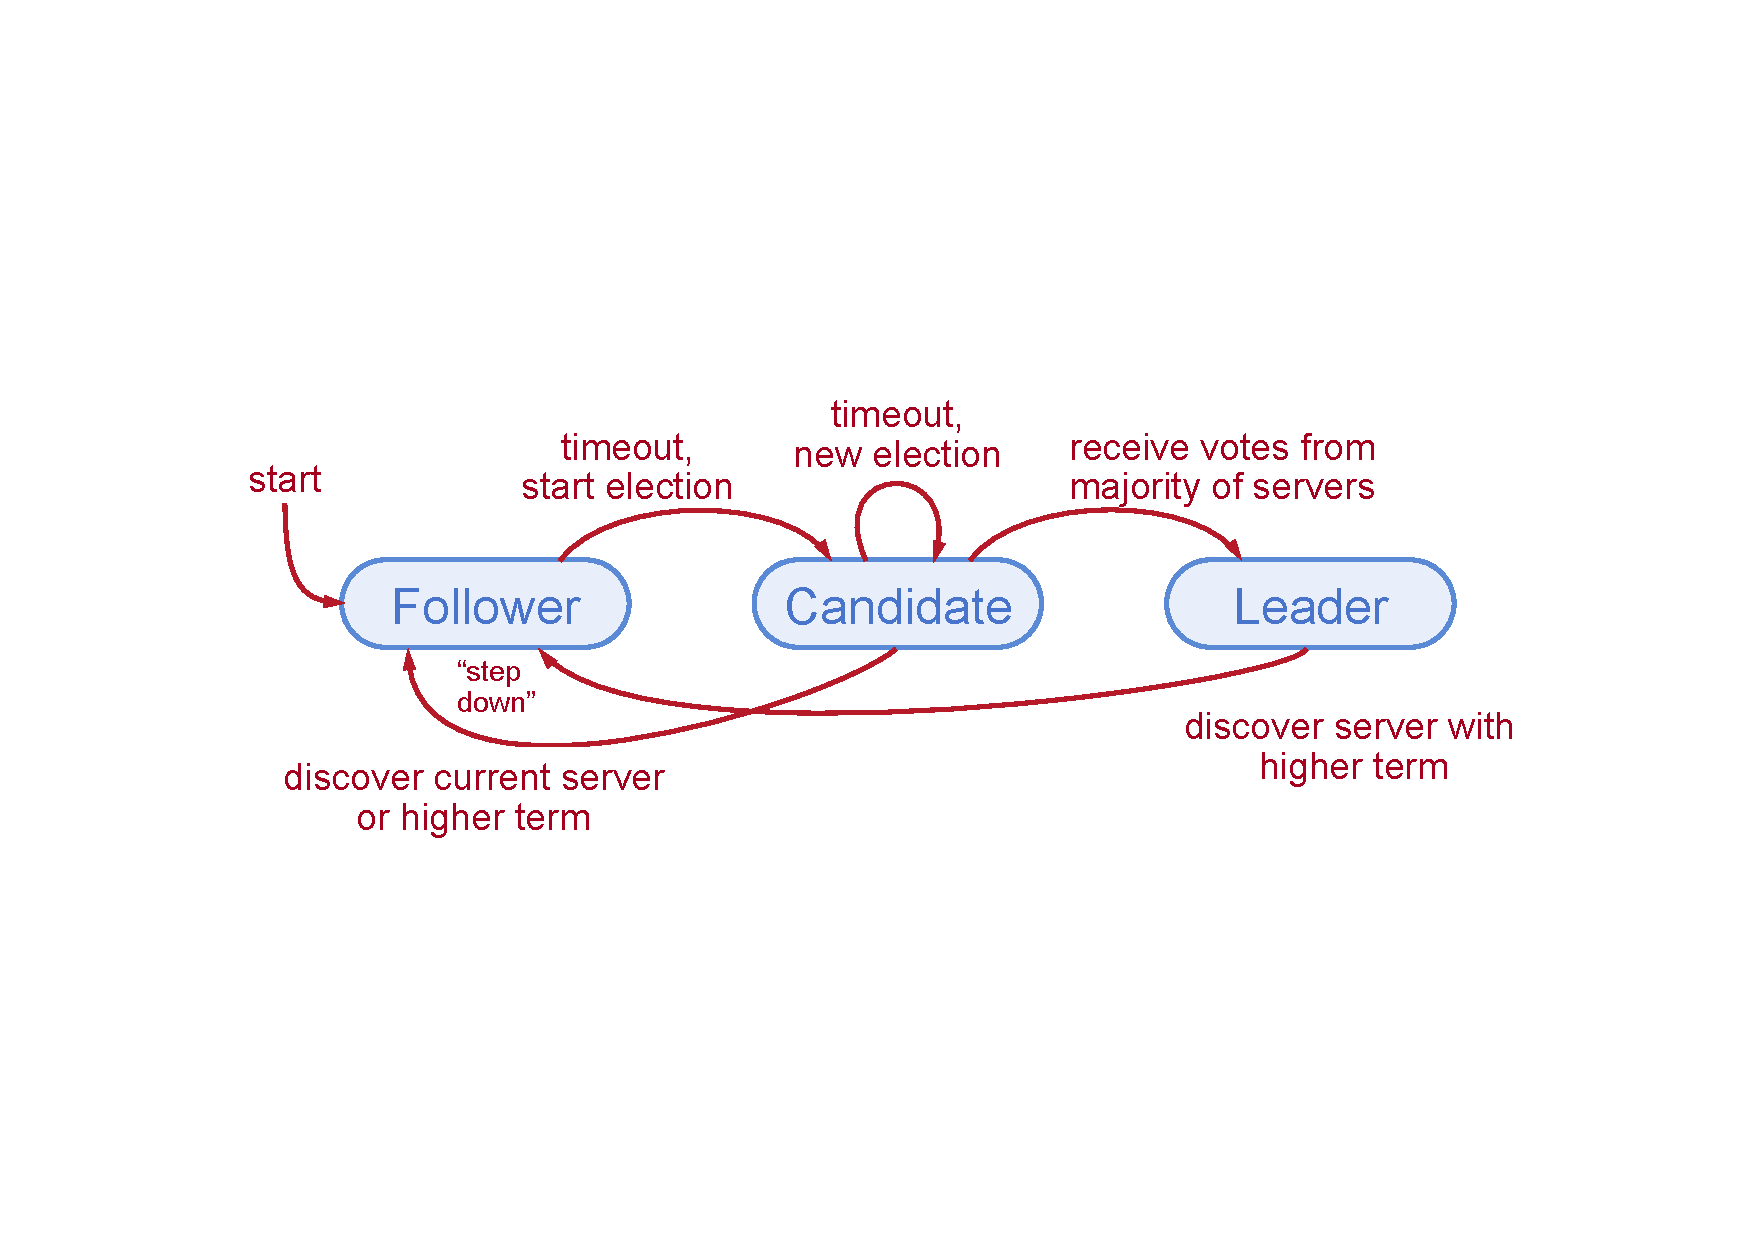
\includegraphics[width=0.90\textwidth]{states.pdf}
\end{center}
\end{frame}

%-------------------------------------------------------------------------
\begin{frame}{Terms}

\begin{center}
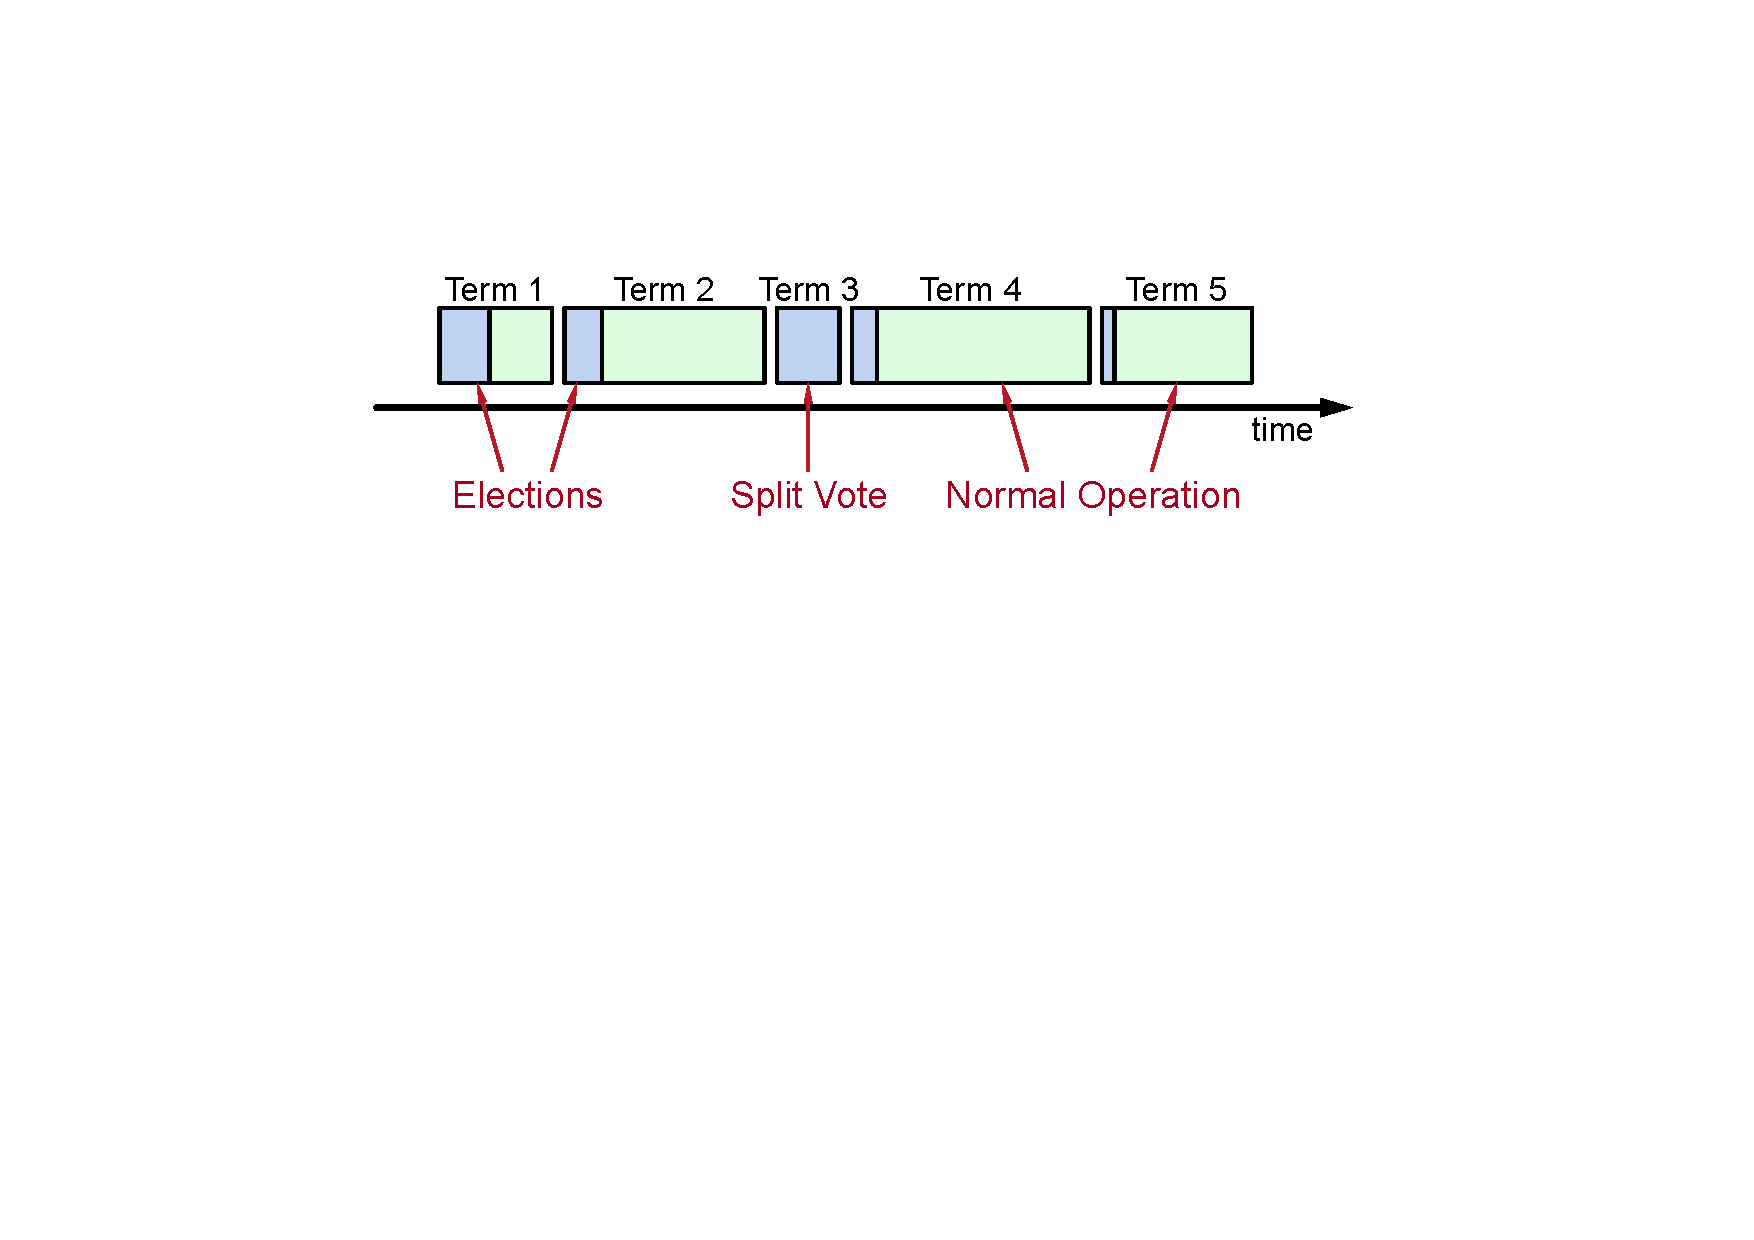
\includegraphics[width=0.70\textwidth]{terms.pdf}
\end{center}

\BIL
\item Time divided into terms:
	\BI
	\item Election
	\item Normal operation under a single leader
	\EI
\item At most one leader per term
\item Some terms have no leader (failed election)
\item Each server maintains \alert{current term} value
\item Key role of terms: \alert{identify obsolete information}
\EIL
		
\end{frame}

%-------------------------------------------------------------------------
\begin{frame}{Server state}

\BB{Persistent state}

Each server persists the following variables to stable storage synchronously before  responding to RPCs:

\bigskip
\begin{tabular}{| P{2cm} | P{9cm} | }
\hline
\RED{\CurrentTerm}	& Latest term server has seen (initialized to 0 on first boot) \\\hline
\RED{\VotedFor} & ID of the candidate that received vote in current term (or null if none) \\\hline
\RED{$\Log[\,]$} & Log entries:	

\medskip
\begin{tabular}{| P{1.5cm} | P{6.7cm} | }
\hline
\RED{\Term} & term when entry was received by leader\\\hline
%\RED{\Index} &	position of entry in the log \\\hline
\RED{\Command} &	command for state machine \\\hline
\end{tabular}

\\\hline
\end{tabular}

\end{frame}

%-------------------------------------------------------------------------
\begin{frame}{Server state}

\BB{Non-persistent state}

\medskip
\begin{tabular}{| P{2.2cm} | P{8.8cm} | }
\hline
\RED{$\State$}	& Current state taken from \Leader, \Candidate, \Follower \\\hline
\RED{$\LeaderVar$} & ID of the leader \\\hline
\RED{$\commitIndex$} & index of highest log entry known to be committed \\\hline
\RED{$\nextIndex[\,]$} & index of next log entry to send to peer \\\hline
\RED{$\matchIndex[\,]$} & index of highest log entry known to be replicated \\\hline
\end{tabular}

\medskip
\BB{Initialization}
{
\vspace{-6pt}
\setlength{\interspacetitleruled}{0pt}%
\setlength{\algotitleheightrule}{0pt}%
\begin{Procedure}
\begin{multicols}{2}
$\CurrentTerm \gets 1$\;
$\VotedFor \gets \Nil$\;
$\Log \gets \{ \}$\;
$\State \gets \Follower$\;
$\LeaderVar \gets \Nil$\;
$\commitIndex \gets 0$\;
$\nextIndex = \{ 1, 1, \ldots, 1 \}$\;
$\matchIndex = \{ 0, 0, \ldots, 0 \}$\;
\end{multicols}
\end{Procedure}
}


\end{frame}



%-------------------------------------------------------------------------
\begin{frame}{RPCs}

Communication between leader and servers happen through two RPCs:
\BIL
\item \AppendRPC
	\BI
	\item Add an entry to the log, \emph{or}
	\item Empty messages used as \alert{heartbeats}
	\item Message tags: \APPENDREQUEST, \APPENDREPLY
	\EI 
\item \VoteRPC
	\BI
	\item Message used by candidates to ask votes and win elections
	\item Message tags: \VOTEREQUEST, \VOTEREPLY
	\EI
\EIL

\end{frame}

%-------------------------------------------------------------------------
\begin{frame}{Hearthbeats and timeouts}

\BIL
\item Servers start up as followers
\item Followers expect to receive RPCs from leaders or candidates
\item Leaders must send empty \AppendRPC RPCs to maintain authority
\item If $\electionTimeout$ time units elapse with no RPCs:
	\BI
	\item Follower assumes leader has crashed
	\item Follower starts new election
	\item Timeouts typically 100-500ms
	\EI
\EIL
	
\end{frame}

\subsection{Elections}

%-------------------------------------------------------------------------
\begin{frame}{Election basics - Election start}

\BEL
\item Set new timeout in range $[\electionTimeout, 2 \cdot \electionTimeout]$
\item Increment current term
\item Change to \RED{Candidate} state
\item Vote for self
\item Send \VoteRPC RPCs to all other servers, retry until either:
	\BI
	\item Receive votes from majority of servers:
		\BI
		\item Become \RED{Leader}
		\item Send \AppendRPC heartbeats to all other servers
		\EI
	\item Receive \AppendRPC from valid leader:
		\BI
		\item Return to \RED{Follower} state
		\EI
	\item No one wins election (election timeout elapses):
		\BI
		\item Start new election
		\EI
	\EI
\EEL

\end{frame}

%-------------------------------------------------------------------------
\begin{frame}{Election - Pseudocode}

\begin{Procedure}
\caption{Election code - executed by process $p$}
\ONTIMEOUT{$\langle \Election \rangle$}{
  \If{$\State \in \{ \Follower, \Candidate \}$}{
  	$t \gets \Random(1.0, 2.0) \cdot \electionTimeout$\;
	\SETTIMEOUT $\langle \Election \rangle$ \AT\ $\Now()+t$\;
	$\CurrentTerm \gets \CurrentTerm+1$\;
	$\State \gets \Candidate$\;
	$\VotedFor \gets p$\;
	$\GrantedVotes \gets \{ p \}$\;
	\ForEach{$q \in \Pi$}{
		\CANCELTIMEOUT $\langle \RPCDue, q \rangle$\;
		\SETTIMEOUT $\langle \RPCDue, q \rangle$ \AT\ $\Now()$\;
	}
  }
}
\end{Procedure}
\end{frame}

%-------------------------------------------------------------------------
\begin{frame}{Election - Pseudocode}

\begin{Procedure}
\caption{RPC timeout code - executed by process $p$}
\ONTIMEOUT{$\langle \RPCDue, q \rangle$}{
  \If{$\State = \Candidate$}{
  	\SETTIMEOUT $\langle \RPCDue, q \rangle$ \AT\ $\Now() + \RPCTimeout$\;
	\SEND $\langle \VOTEREQUEST, \CurrentTerm \rangle$ \TO\ $q$
  }
}

\end{Procedure}
\end{frame}

%-------------------------------------------------------------------------
\begin{frame}{Election - Pseudocode}

\begin{Procedure}
\caption{Election code - executed by process $p$}
\ONRECEIVE{$\langle \VOTEREQUEST, \Term \rangle$ \FROM $q$}{
  \If{$\Term > \CurrentTerm$}{
    $\StepDown(\Term)$\;
  }
  \If{$\Term = \CurrentTerm$ \AND\ $\VotedFor \in \{ q, \Nil \}$}{
	$\VotedFor \gets q$\;
  	$t \gets \Random(1.0, 2.0) \cdot \electionTimeout$\;
	\SETTIMEOUT $\langle \Election \rangle$ \AT\ $\Now()+t$\;
  }
  \SEND $\langle \VOTEREPLY, \Term, \VotedFor \rangle$\;
}

\end{Procedure}
\end{frame}


%-------------------------------------------------------------------------
\begin{frame}{Election - Pseudocode}

\begin{Procedure}
\caption{Election code - executed by process $p$}
\ONRECEIVE{$\langle \VOTEREPLY, \Term, \Vote \rangle$ \FROM $q$}{
  \If{$\Term > \CurrentTerm$}{
    $\StepDown(\Term)$\;
  }
  \If{$\Term = \CurrentTerm$ \AND\ $\State = \Candidate$}{
  	\If{$\Vote = p$}{
  		$\GrantedVotes \gets \GrantedVotes \cup \{ q\}$\;
	}
	\CANCELTIMEOUT $\langle \RPCDue, q \rangle$\;
	\If{$|\GrantedVotes|> |\Pi|/2$}{
		$\State \gets \Leader$\;
		$\LeaderVar \gets p$\;
		\ForEach{$q \in P-\{p\}$}{
			$\SendAppendEntries(q)$\;
		}
	}
  }
}

\end{Procedure}
\end{frame}


\begin{frame}{Election - Pseudocode}

{
\setlength{\interspacetitleruled}{0pt}%
\setlength{\algotitleheightrule}{0pt}%
\begin{Procedure}
\PROCEDURE{$\StepDown(\Term)$}{
  $\CurrentTerm \gets \Term$\;
  $\State \gets \Follower$\;
  $\VotedFor \gets \Nil$\; 
  $t \gets \Random(1.0, 2.0) \cdot \electionTimeout$\;
  \SETTIMEOUT $\langle \Election \rangle$ \AT\ $\Now()+t$\;
}
\end{Procedure}
}
\end{frame}

%-------------------------------------------------------------------------
\begin{frame}{Election - Correctness}
	
\BB{\alert{Safety}:  allow at most one winner per term}
	\BI
	\item Each server gives out only one vote per term (persist on disk)	
	\item Two different candidates can't accumulate majorities in same term
	\EI
	\begin{center}
	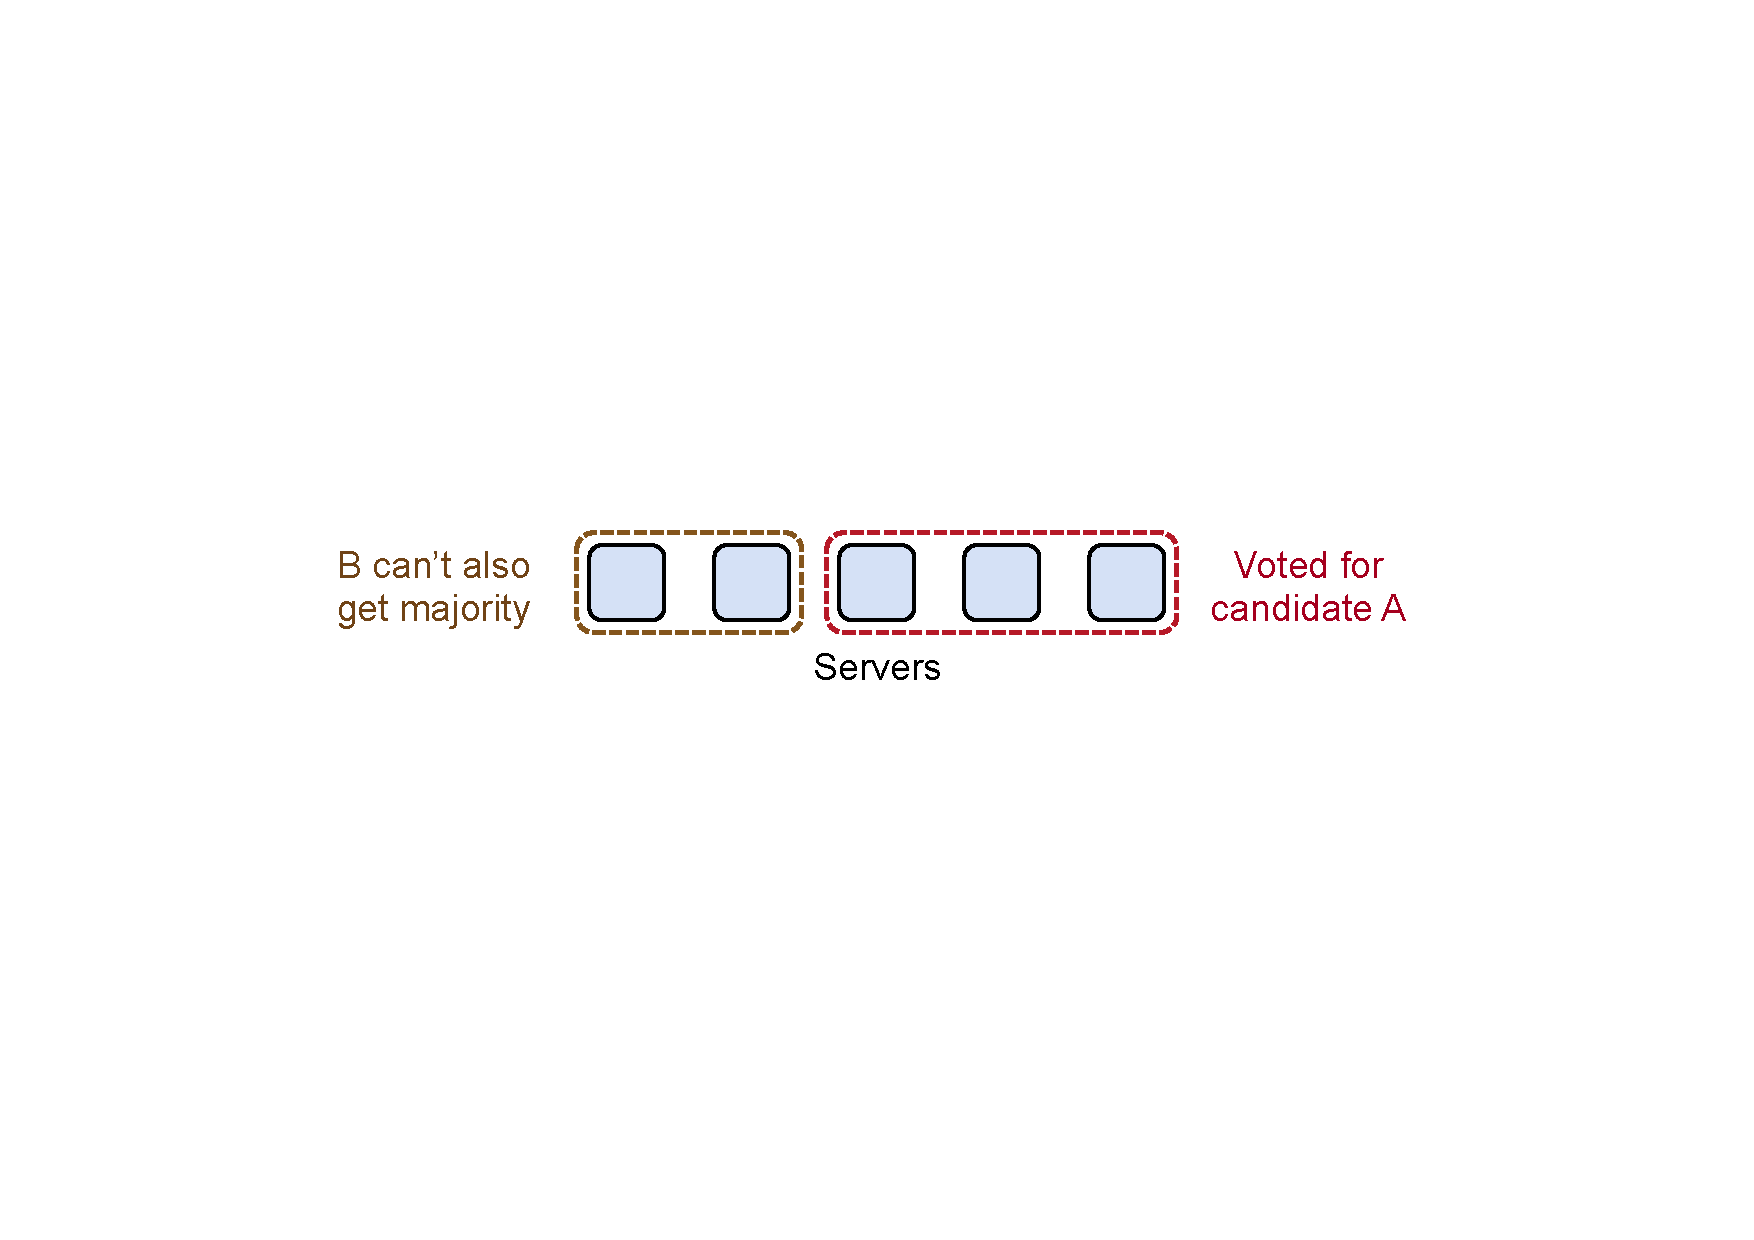
\includegraphics[width=0.9\textwidth]{majority}
	\end{center}

\BB{\alert{Liveness}: some candidate must eventually win}
	\BI
	\item Choose election timeouts randomly in $[\electionTimeout, 2 \cdot \electionTimeout]$
	\item One server usually times out and wins election before others wake up
	\item Works well if $\electionTimeout >>$ broadcast time
	\EI

	
\end{frame}

\begin{frame}{Randomize timeouts}
\BI
\item How much randomization is needed to avoid split votes?
\item Conservatively, use random range $\approx 10\times$ network latency
\EI

\begin{center}
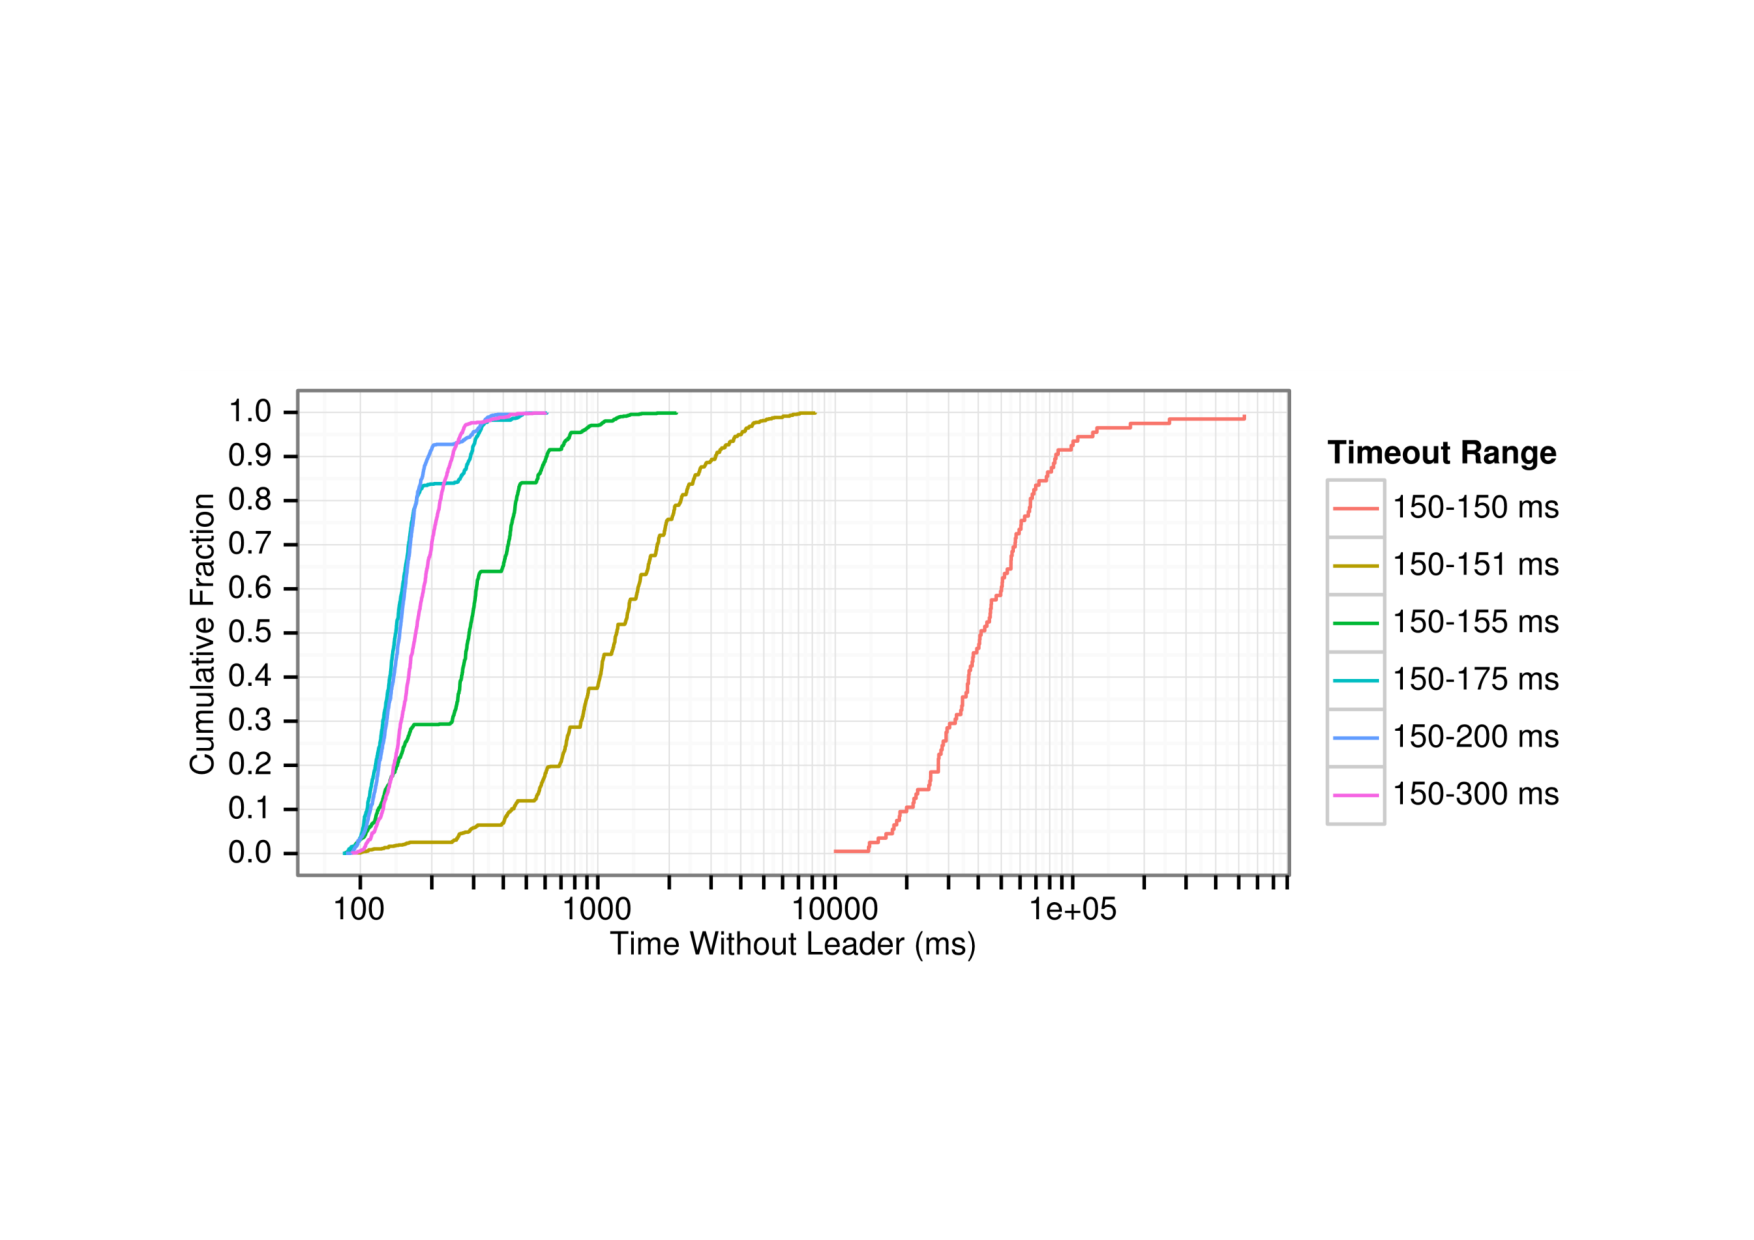
\includegraphics[width=1.0\textwidth]{randomization}
\end{center}

\end{frame}

\begin{frame}{Log structure}

\begin{center}
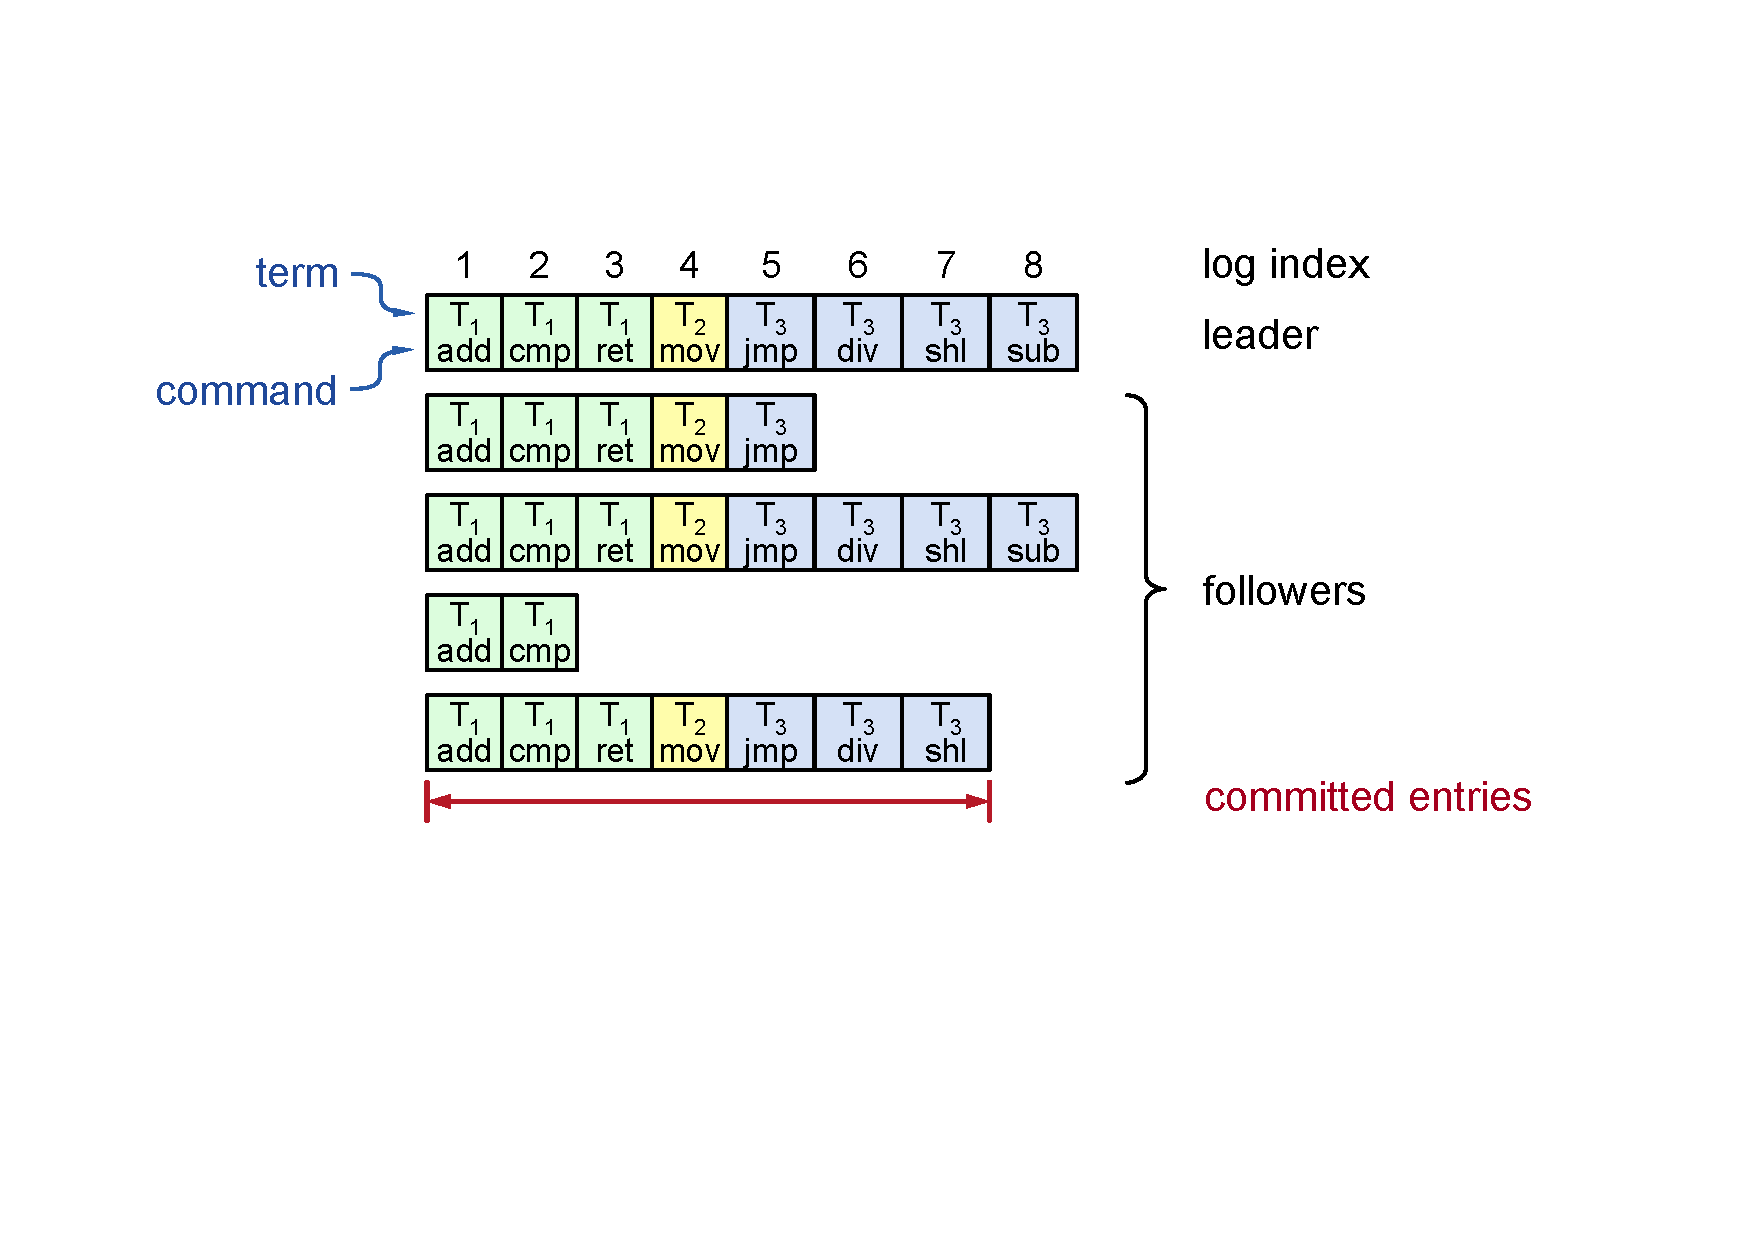
\includegraphics[width=0.9\textwidth]{log}
\end{center}

\BI
\item Log stored on stable storage (disk); survives crashes
\item Entry \alert{committed} if \alert{known} to be stored on majority of servers
\item Durable, will eventually be executed by state machines
\EI
	
\end{frame}

\subsection{Normal operation}


\begin{frame}{Normal operation}
\BIL
\item Client sends command to leader
\item Leader appends command to its log
\EIL

\begin{Procedure}
\caption{Normal operation code executed by process $p$}
\UPON{\RECEIVE $\langle \Request, \Command \rangle$ \FROM\ client}{
	\If{$\State = \Leader$}{
  		$\Log.\Append(\CurrentTerm, \Command)$\;
		\ForEach{$q \in P-\{p\}$}{
			$\SendAppendEntries(q)$\;
		}
	}
}
\end{Procedure}

\end{frame}

\begin{frame}{Normal operation}
\BIL
\item Leader sends \AppendRPC RPCs to followers
\item Once new entry committed:
	\BI
	\item Leader passes command to its state machine, returns result to client
	\item Leader notifies followers of committed entries in subsequent AppendEntries RPCs
	\item Followers pass committed commands to their state machines
	\EI
\item Crashed/slow followers?
	\BI
	\item Leader retries RPCs until they succeed
	\item Performance is optimal in common case: one successful RPC to any majority of servers
	\EI
\EIL

\end{frame}

\begin{frame}{Normal operation}

\begin{Procedure}
\caption{RPC timeout code executed by process $p$}
\ONTIMEOUT{$\langle \RPCDue, q \rangle$}{
  \If{$\State = \Candidate$}{
  	\SETTIMEOUT $\langle \RPCDue, q \rangle$ \AT\ $\Now() + \RPCTimeout$\;
	\SEND $\langle \VOTEREQUEST, \CurrentTerm \rangle$ \TO\ $q$
  }
\alert{
  \If{$\State = \Leader$}{
	$\SendAppendEntries(q)$\;
  }
}
}
\end{Procedure}
\end{frame}



\begin{frame}{How to send append entries}

{
\setlength{\interspacetitleruled}{0pt}%
\setlength{\algotitleheightrule}{0pt}%
\begin{Procedure}
\PROCEDURE{$\SendAppendEntries(q)$}{
  	\SETTIMEOUT $\langle \RPCDue, q \rangle$ \AT\ $\Now() + \electionTimeout/2$\;
	$\lastIndex \gets \textrm{choose in} [\nextIndex[q],\Log.\Length()]$\;
	$\nextIndex[q] = \lastIndex$\;
	\SEND $\langle \Term, \lastIndex-1, \Log[\lastIndex[q]-1].\Term$\;
	\hspace{1.1cm}$\Log[\lastIndex \ldots \Log.\Length()], \commitIndex \rangle$ \TO $q$\;
}
\end{Procedure}
}
\end{frame}

\begin{frame}{Log consistency}

\begin{block}{Consistency in logs}
\BIL
\item If log entries on different servers have same index and term:
\BI
\item They store the same command
\item The logs are identical in all preceding entries
\EI
\item If a given entry is committed, all preceding entries are also committed
\EIL
\end{block}

\smallskip
\begin{center}
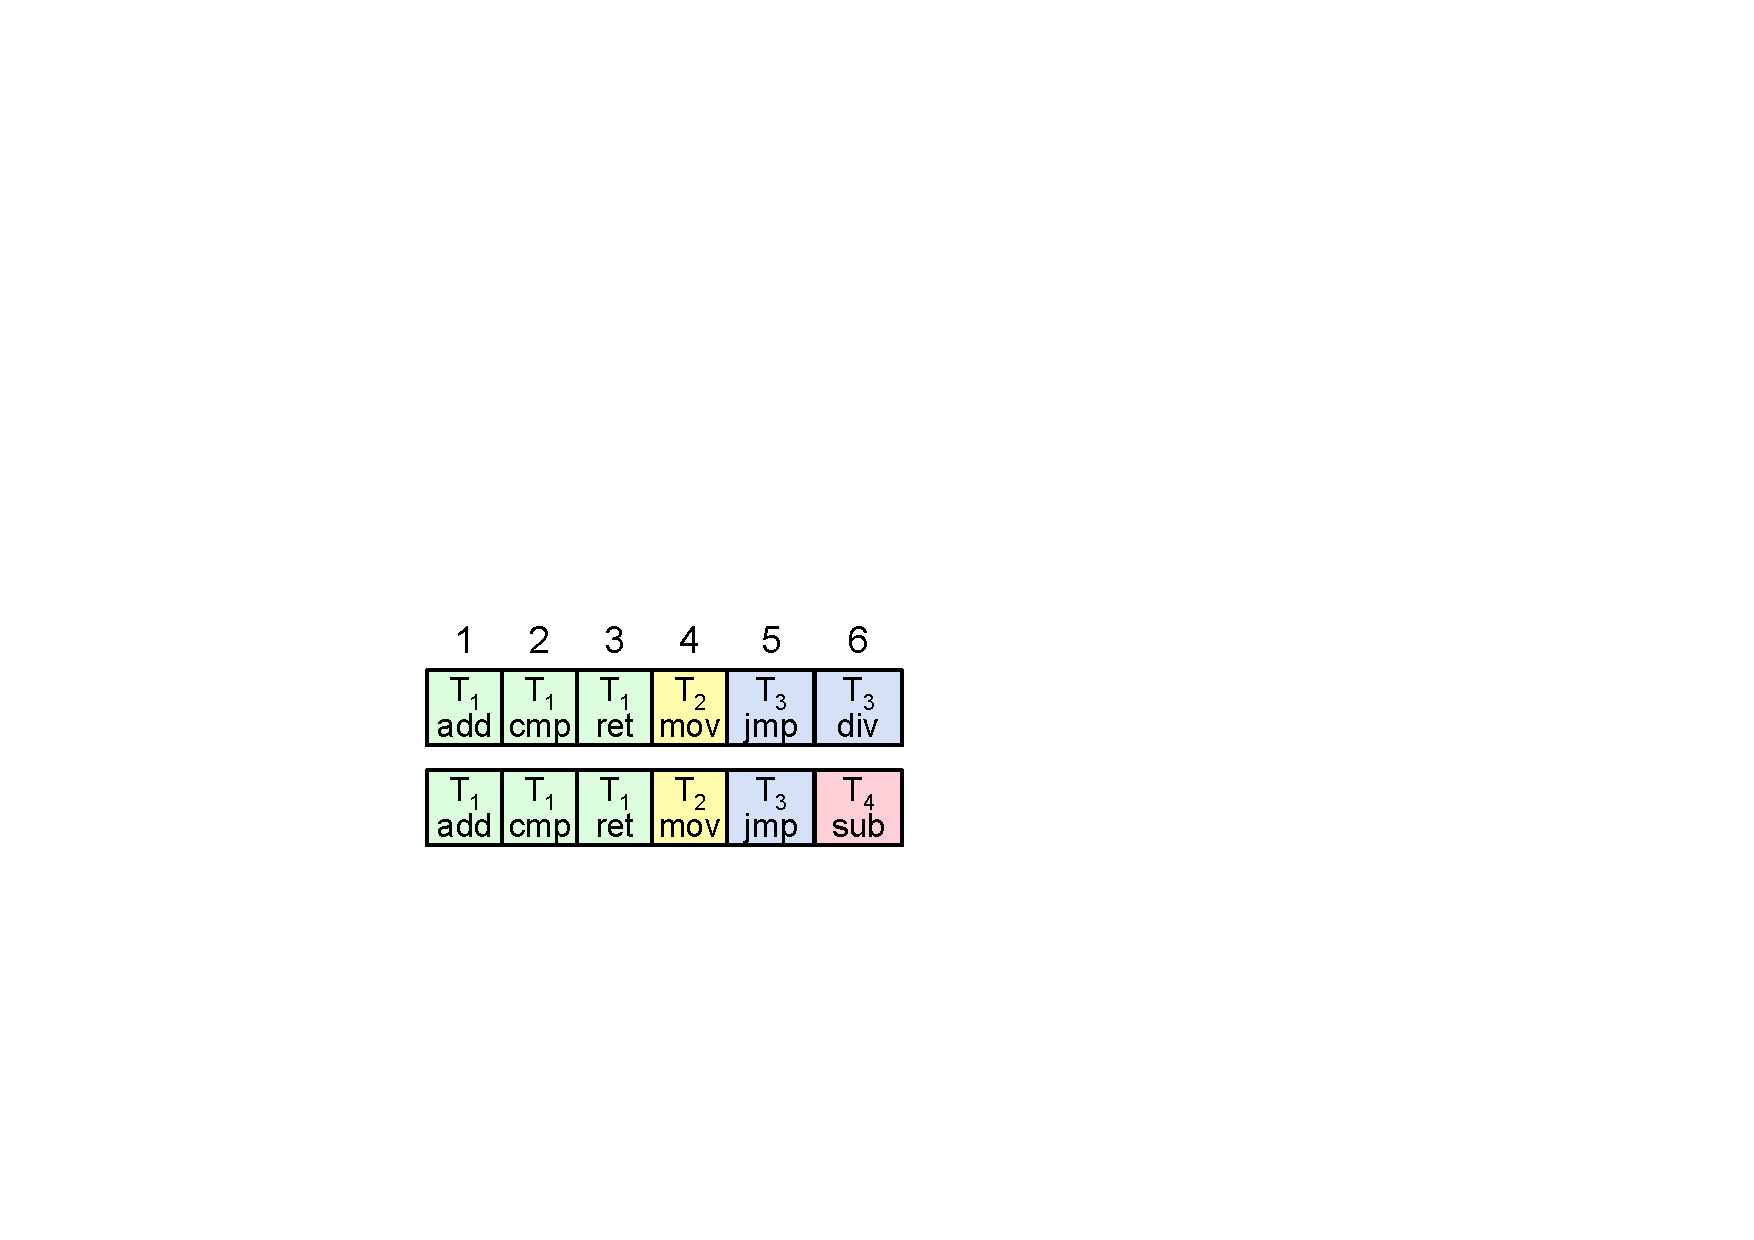
\includegraphics[width=0.5\textwidth]{log-consistency}
\end{center}


\end{frame}



\begin{frame}{\AppendRPC Consistency Check}
	
\BI
\item Each \AppendRPC RPC contains index, term of entry preceding new ones
\item Follower must contain matching entry;  otherwise it rejects request
\item Implements an \alert{induction} step, ensures coherency
\EI

\smallskip
\begin{center}
\begin{overprint}
\onslide<1|handout:1>
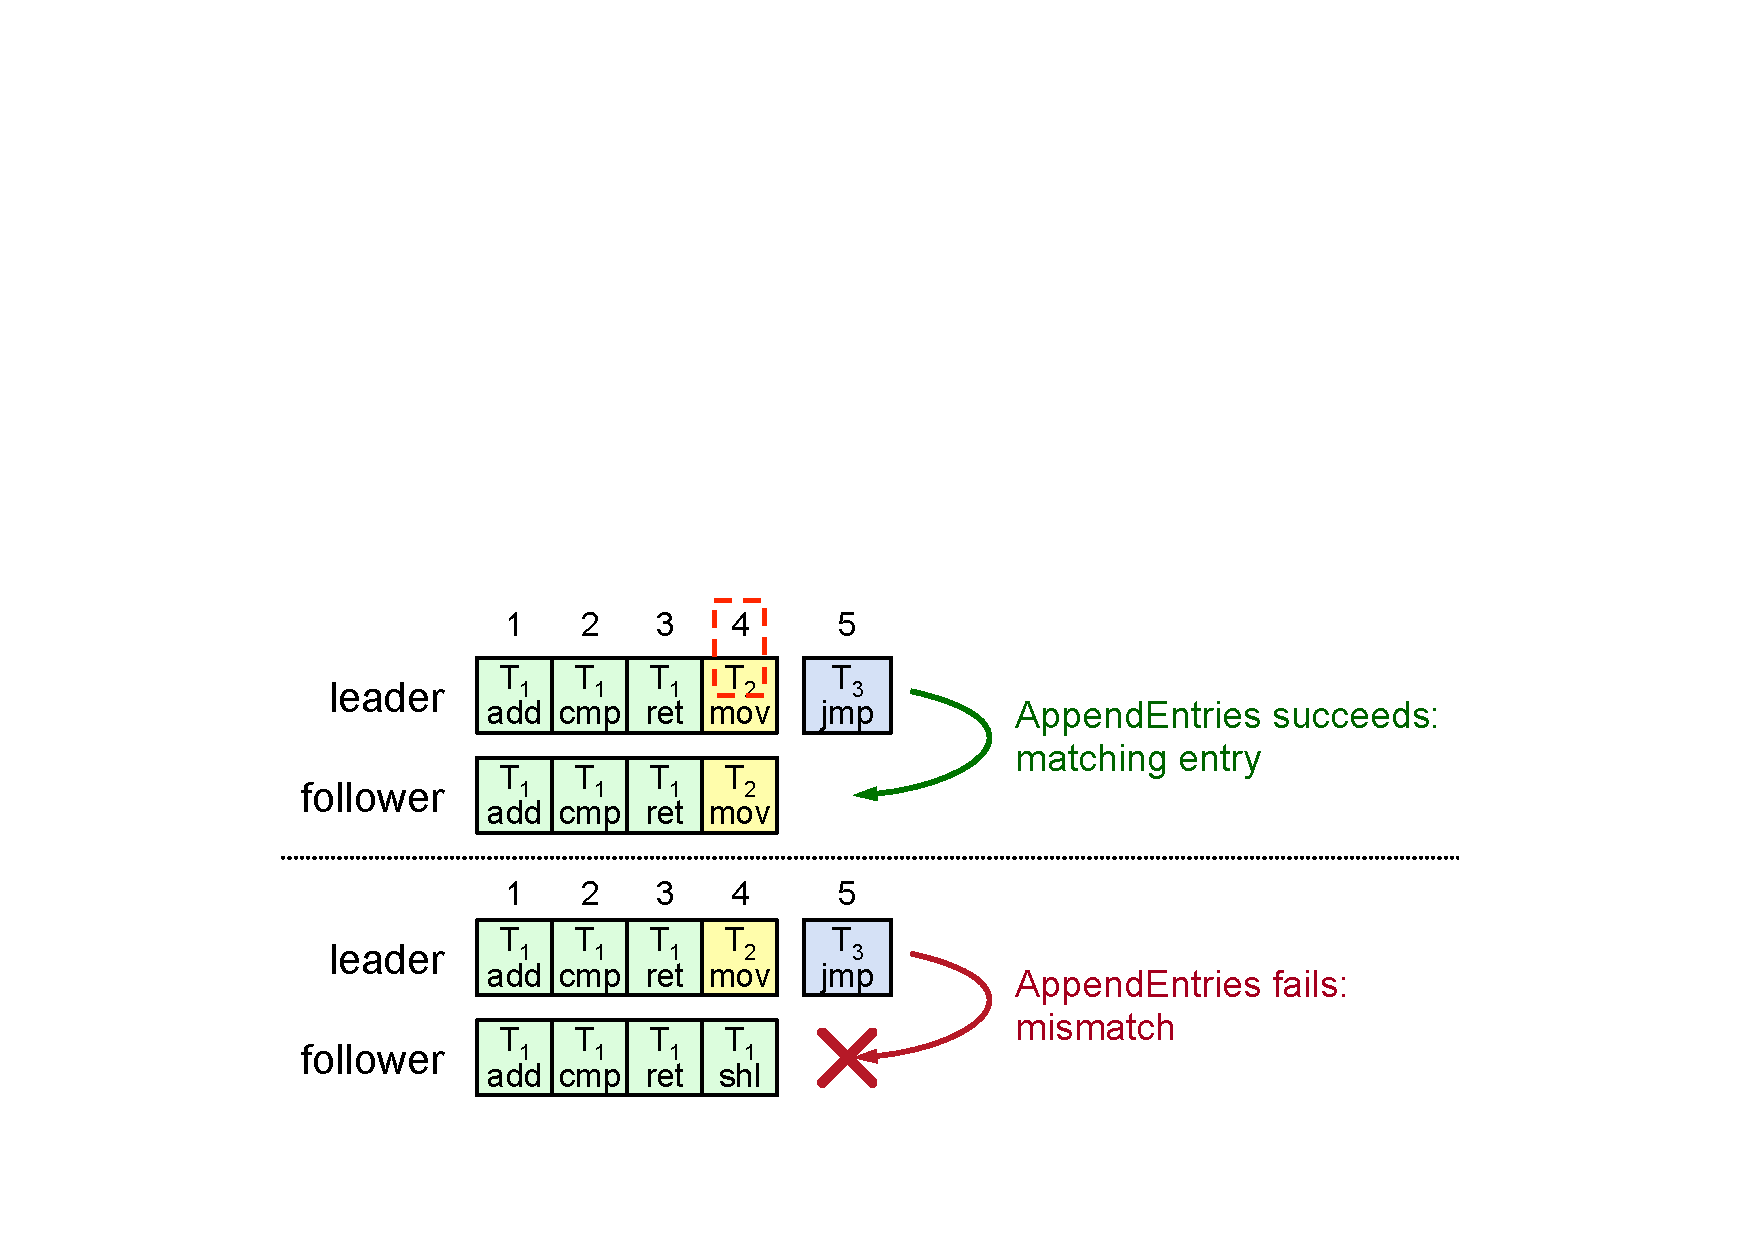
\includegraphics[width=0.8\textwidth,page=1]{consistency-check}
\onslide<2|handout:2>
\includegraphics[width=0.8\textwidth,page=2]{consistency-check}
\end{overprint}
\end{center}

\end{frame}

%-------------------------------------------------------------------------
\begin{frame}[shrink=5]{Normal operation - Pseudocode}

\begin{Procedure}
\caption{Normal operation code - executed by process $p$}
\ONRECEIVE{$\langle \APPENDREQUEST, \Term, \prevIndex, \prevTerm, \Entries, \commitIndex \rangle$ \FROM $q$}{
  \If{$\Term > \CurrentTerm$}{
    $\StepDown(\Term)$\;
  }
  \eIf{$\Term < \CurrentTerm$}{
    \SEND $\langle \APPENDREPLY, \CurrentTerm, \FALSE \rangle$ \TO\ $q$
  }{
    $\Index \gets 0$\;
  	$\Success \gets \prevIndex=0$\ \OR\ $(\prevIndex \leq \Log.\Length()$\ \AND\
	\qquad\qquad $\Log[\prevIndex].\Term = \prevTerm)$\;
	\If{$\Success$}{
		$\StoreEntries(\prevIndex, \Entries, \commitIndex)$\;
	}
	\SEND $\langle  \APPENDREPLY, \CurrentTerm, \Success, \Index \rangle$
  }
}
\end{Procedure}
\end{frame}

%-------------------------------------------------------------------------
\begin{frame}{At beginning of new leader's term}

\BI
\item Old leader may have left entries partially replicated
\item No special steps by new leader: just start normal operation
\item Leader's log is “the truth”
\item Will eventually make follower's logs identical to leader's
\item Multiple crashes can leave many extraneous log entries
\EI

\begin{center}
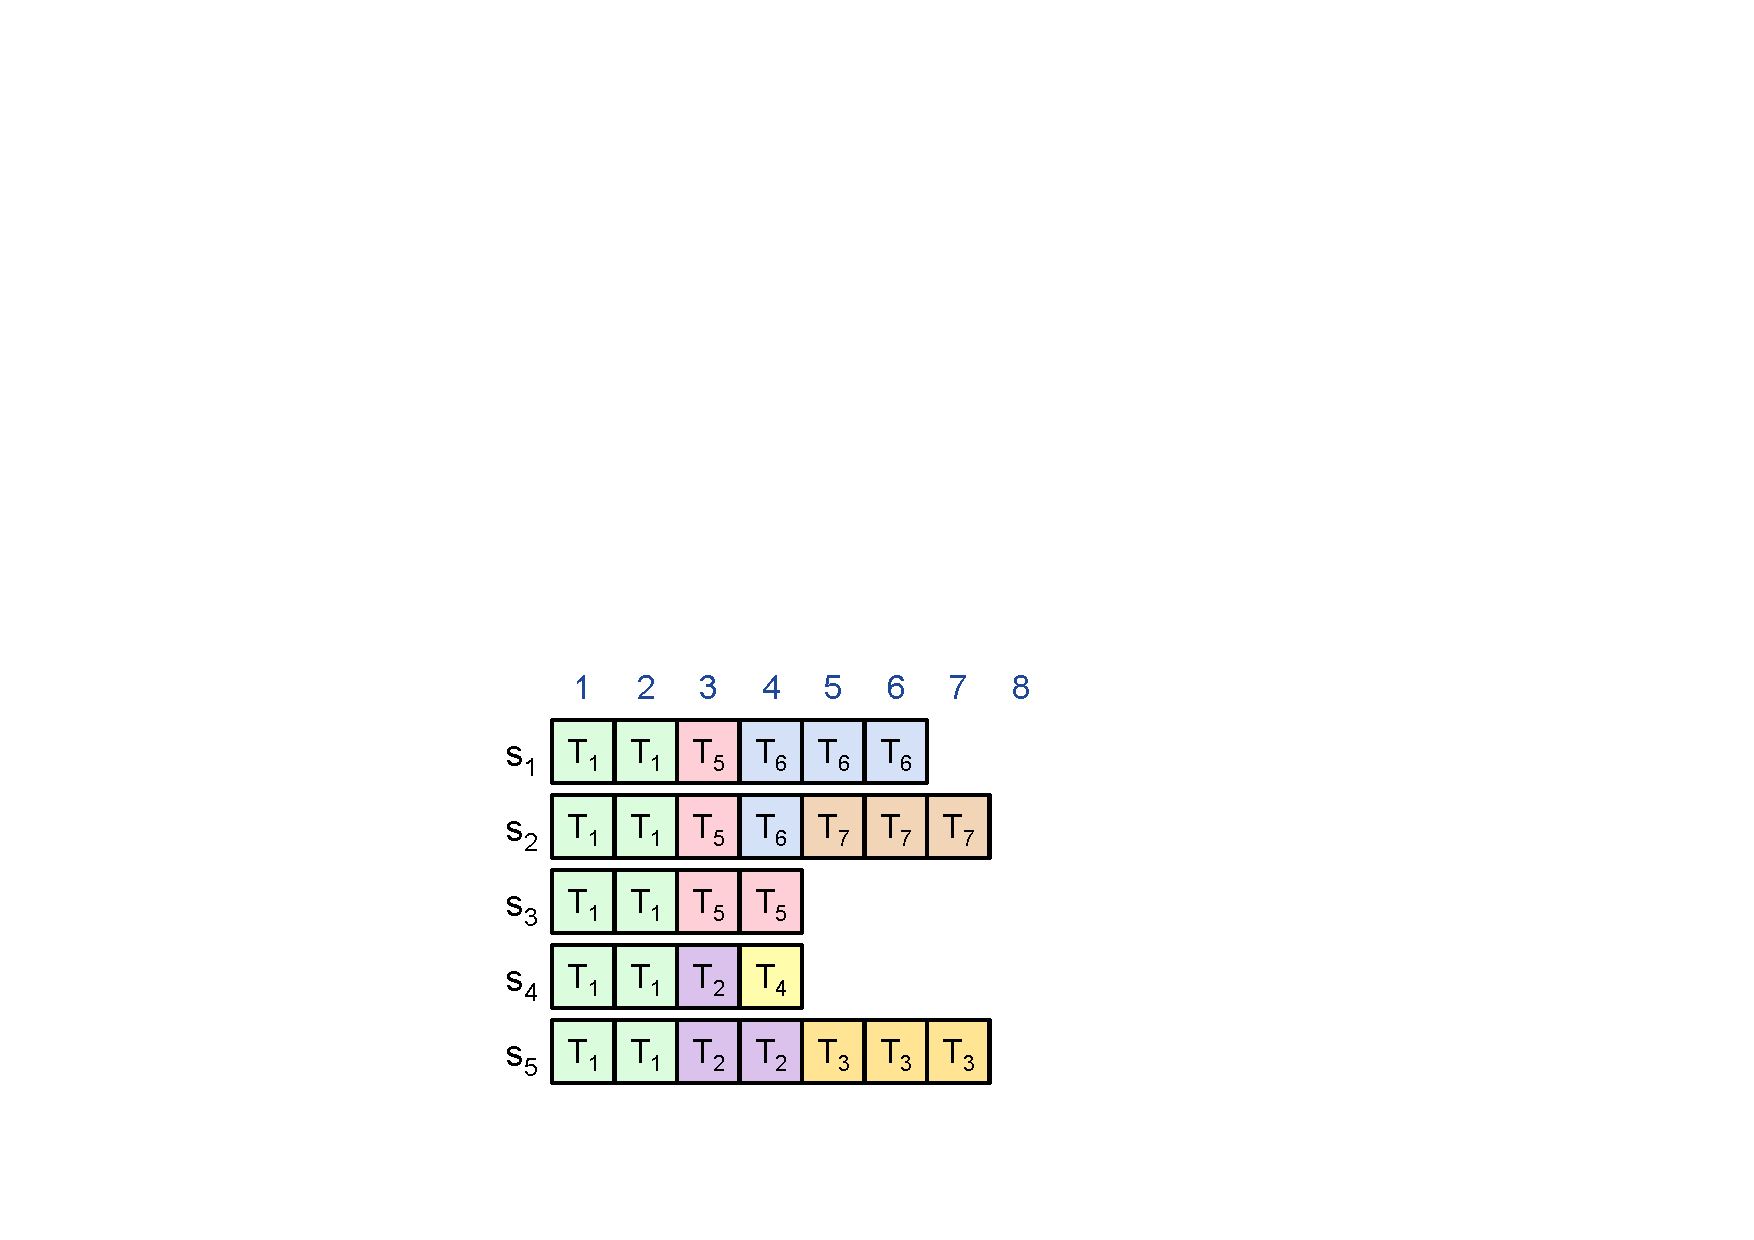
\includegraphics[width=0.5\textwidth]{leader-changes}
\end{center}

\end{frame}


%-------------------------------------------------------------------------
\begin{frame}{Safety Requirement}
	
\BB{\centering Once a log entry has been applied to a state machine, no other \\
state machine must apply a different value for that log entry}

\BIL
\item Raft safety property:
	\BI
	\item If a leader has decided that a log entry is committed, that entry will be present in the logs of all future leaders
	\item This guarantees the safety requirement
	\EI
\item Leaders never overwrite entries in their logs
	\BI
	\item Only entries in the leader's log can be committed
	\item Entries must be committed before applying to state machine
	\EI
\EIL

\begin{center}
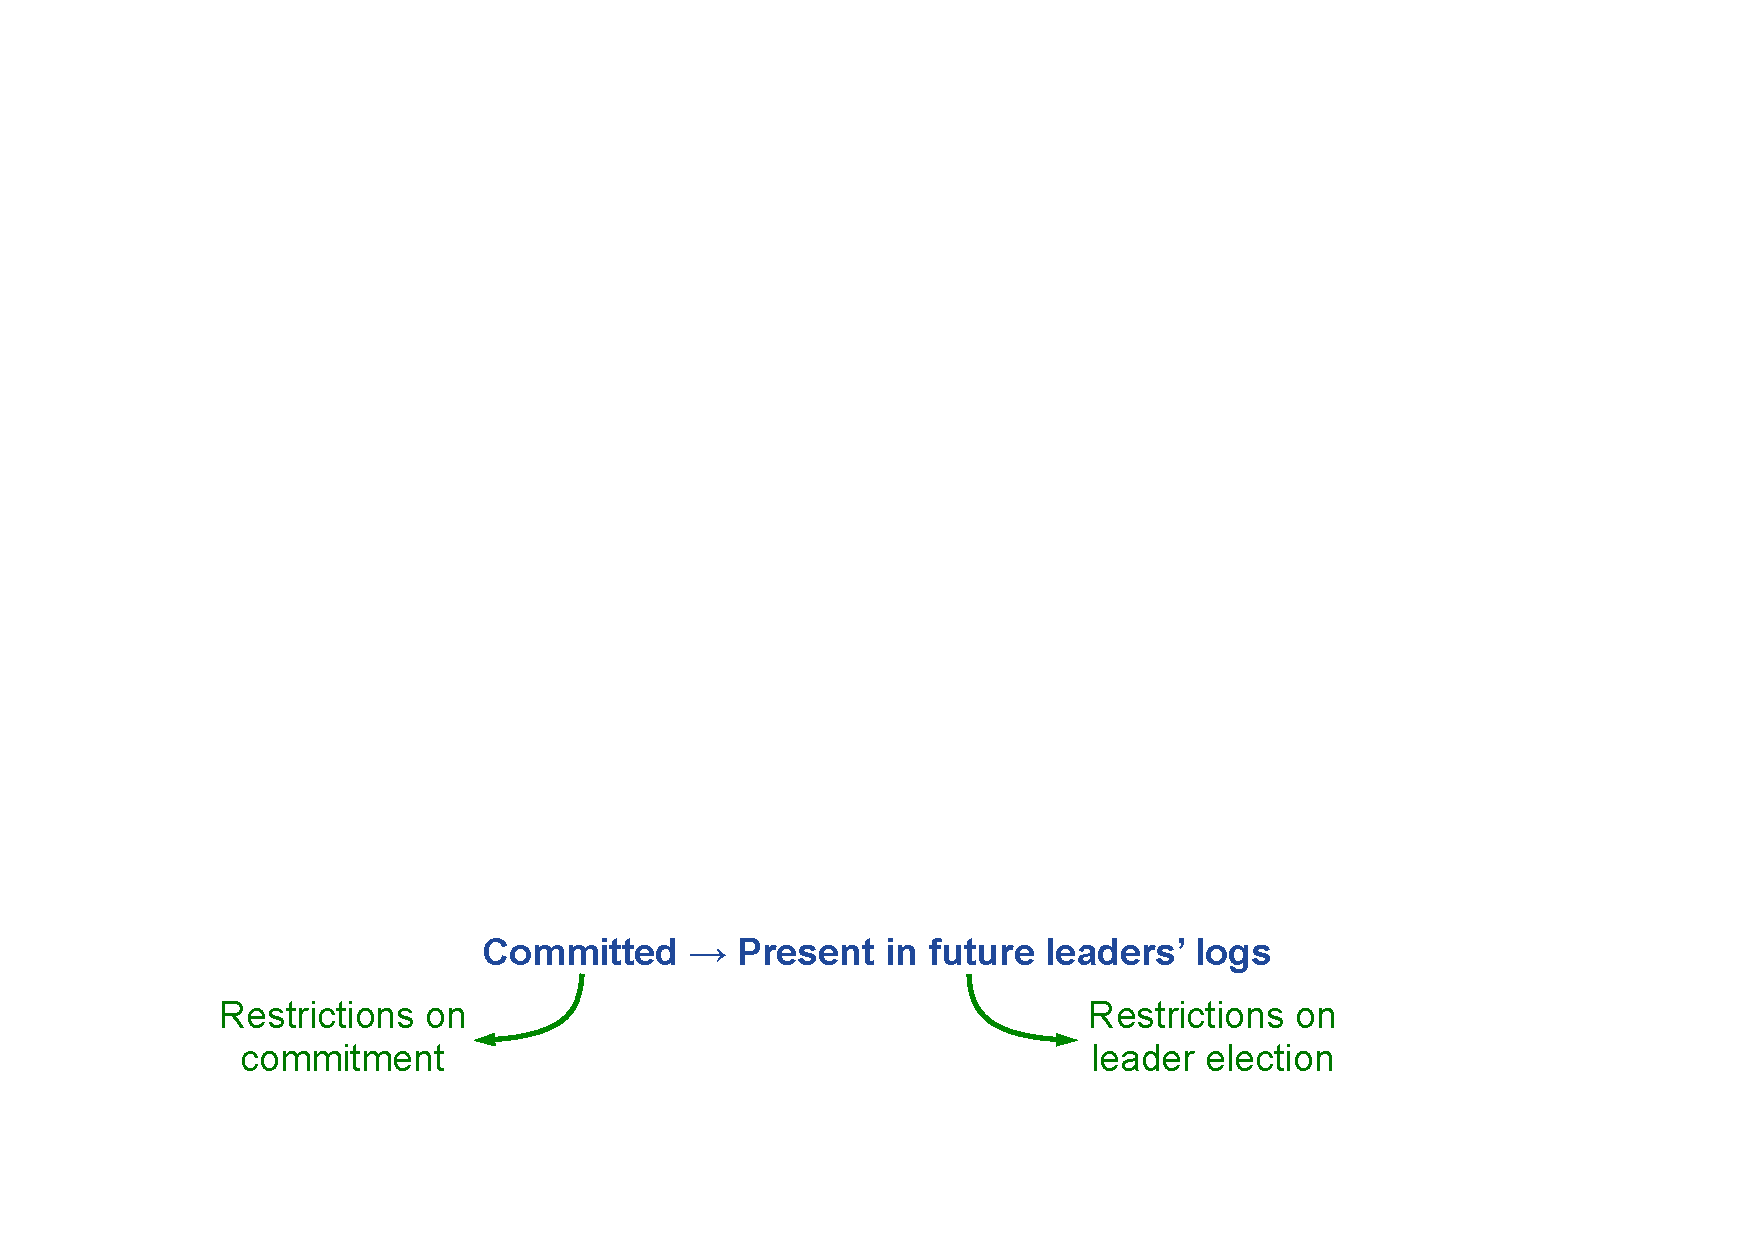
\includegraphics[width=0.9\textwidth]{safety}
\end{center}


\end{frame}


%-------------------------------------------------------------------------
\begin{frame}{Picking the Best Leader}
	
\begin{columns}[T]
\begin{column}{0.38\textwidth}
\BIL
\item Can't tell which entries are committed!
\EIL
\end{column}
\begin{column}{0.6\textwidth}
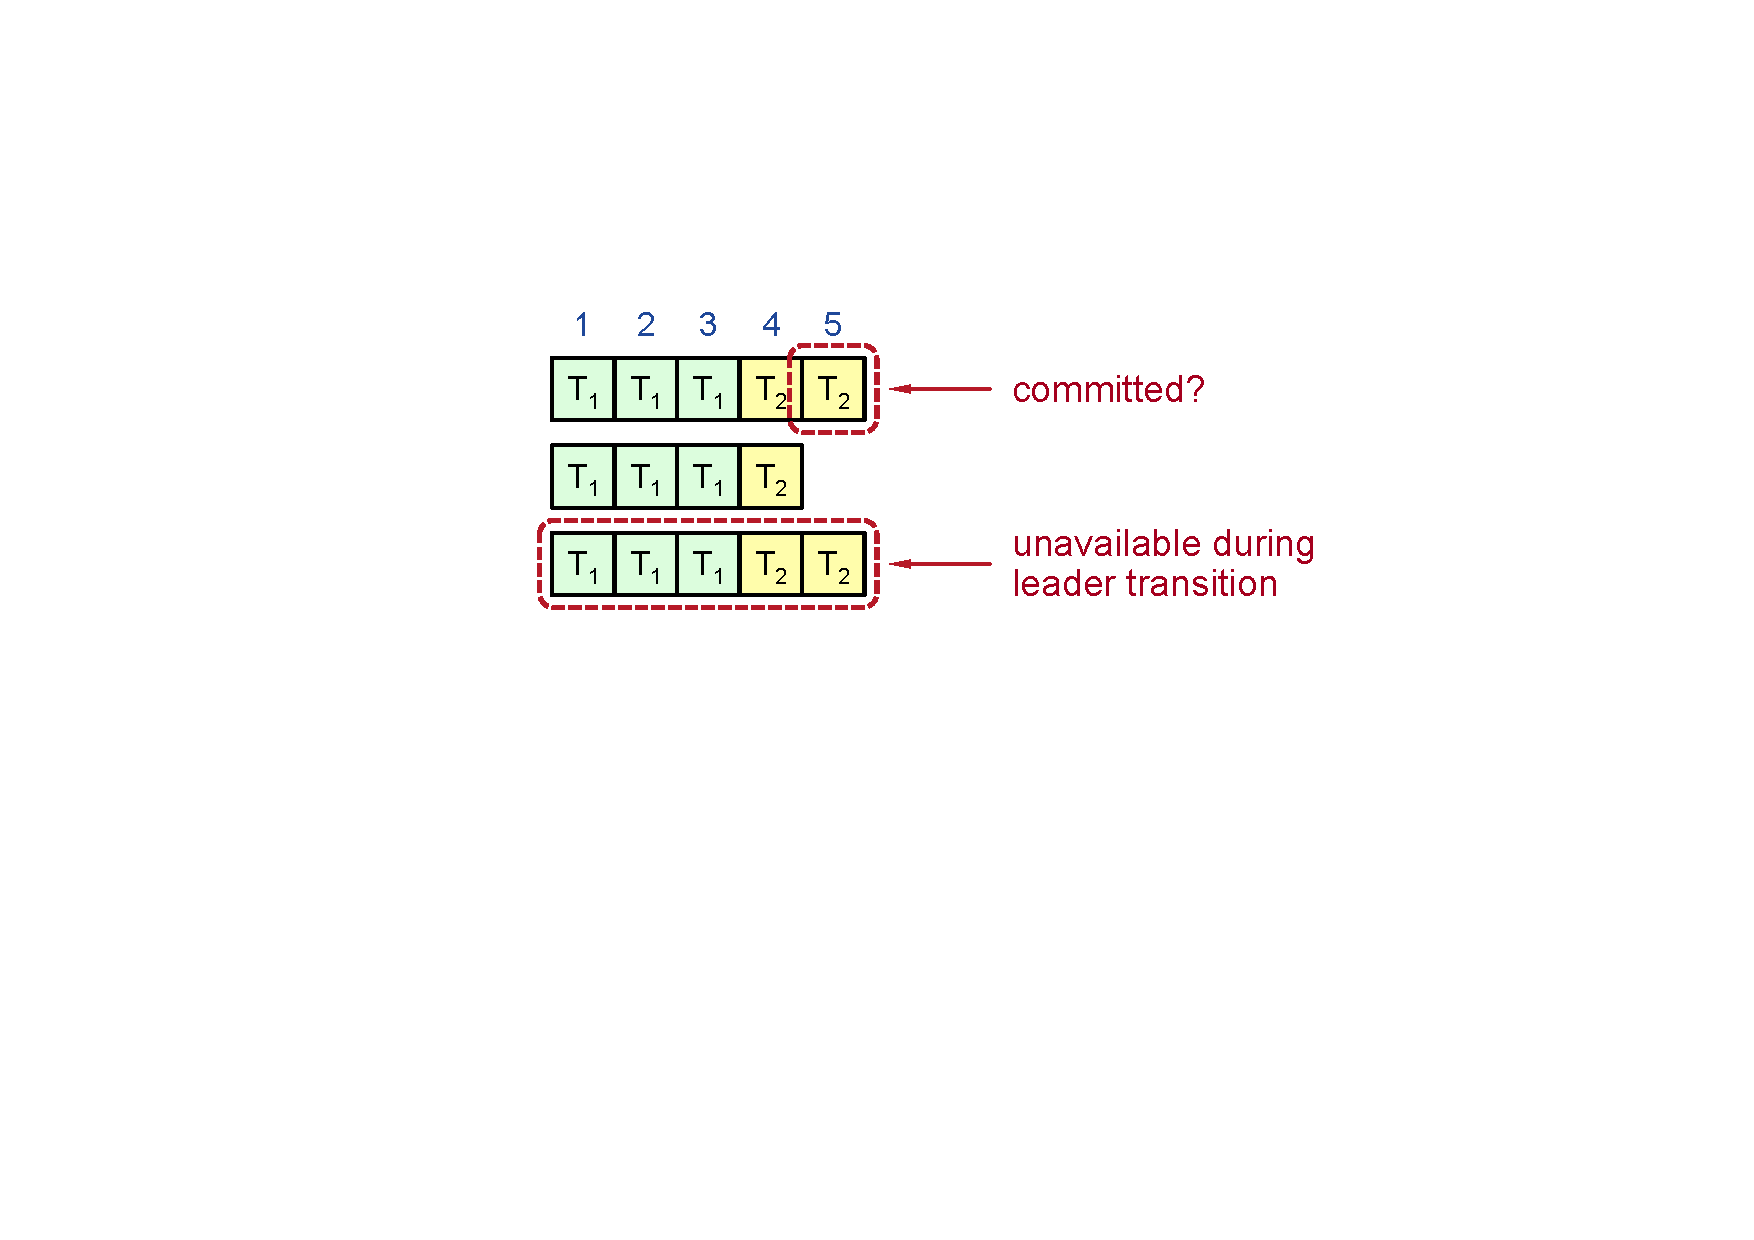
\includegraphics[width=\textwidth]{iscommitted}
\end{column}
\end{columns}
\BIL
%\item Can't tell which entries are committed!
\item During elections, choose candidate with log most likely to contain all committed entries
\smallskip
\BIL
\item Candidates include index \& term of last log entry in \VOTEREQUEST
\item Voting server $V$ \alert{denies} vote if its log is “more complete”:
{\footnotesize $(\lastTerm_C < \lastTerm_V)\ \OR\ $\\
$(\lastTerm_C = \lastTerm_V \ \AND\ \lastIndex_C < \lastIndex_V)$}
\item Leader will have “most complete” log among electing majority
\EI
\EIL

\end{frame}

%-------------------------------------------------------------------------
\begin{frame}{Election - Modified pseudocode}

\begin{Procedure}
\caption{RPC timeout code - executed by process $p$}
\ONTIMEOUT{$\langle \RPCDue, q \rangle$}{
  \If{$\State = \Candidate$}{
  	\SETTIMEOUT $\langle \RPCDue, q \rangle$ \AT\ $\Now() + \RPCTimeout$\;
	\alert{$\lastTerm \gets \Log[\Log.\Length()].\Term$}\;
	\alert{$\lastIndex \gets \Log.\Length()$}\;
	\SEND $\langle \VOTEREQUEST, \CurrentTerm, \alert{\lastTerm, \lastIndex} \rangle$ \TO\ $q$
  }
  \If{$\State = \Leader$}{
  	\SETTIMEOUT $\langle \RPCDue, q \rangle$ \AT\ $\Now() + \electionTimeout/2$\;
	$\SendAppendEntries(q)$\;
  }
}

\end{Procedure}
\end{frame}

%-------------------------------------------------------------------------
\begin{frame}{Election - Modified pseudocode}

\begin{Procedure}
\caption{Election code - executed by process $p$}
\ONRECEIVE{$\langle \VOTEREQUEST, \Term, \alert{\lastTerm, \lastIndex} \rangle$ \FROM $q$}{
  \If{$\Term > \CurrentTerm$}{
    $\StepDown(\Term)$\;
  }
  \If{$\Term = \CurrentTerm$\ \AND\
  	$\VotedFor \in \{ q, \Nil \}$\ \alert{\AND}\ \\
    \alert{$\quad (\lastTerm > \Log[\Log.\Length()].\Term$\ \OR\ } \\
	\alert{$\quad (\lastTerm = \Log[\Log.\Length()].\Term$\ \AND\ $\lastIndex \geq \Log.\Length() )~)$}
  }{
	$\VotedFor \gets q$\;
  	$t \gets \Random(1.0, 2.0) \cdot \electionTimeout$\;
	\SETTIMEOUT $\langle \Election \rangle$ \AT\ $\Now()+t$\;
  }
  \SEND $\langle \VOTEREPLY, \Term, \VotedFor \rangle$\;
}

\end{Procedure}
\end{frame}

%-------------------------------------------------------------------------
\begin{frame}[t]{Committing Entry from Current Term}

\BB{Case 1/2: Leader decides entry in current term is committed}

\begin{center}
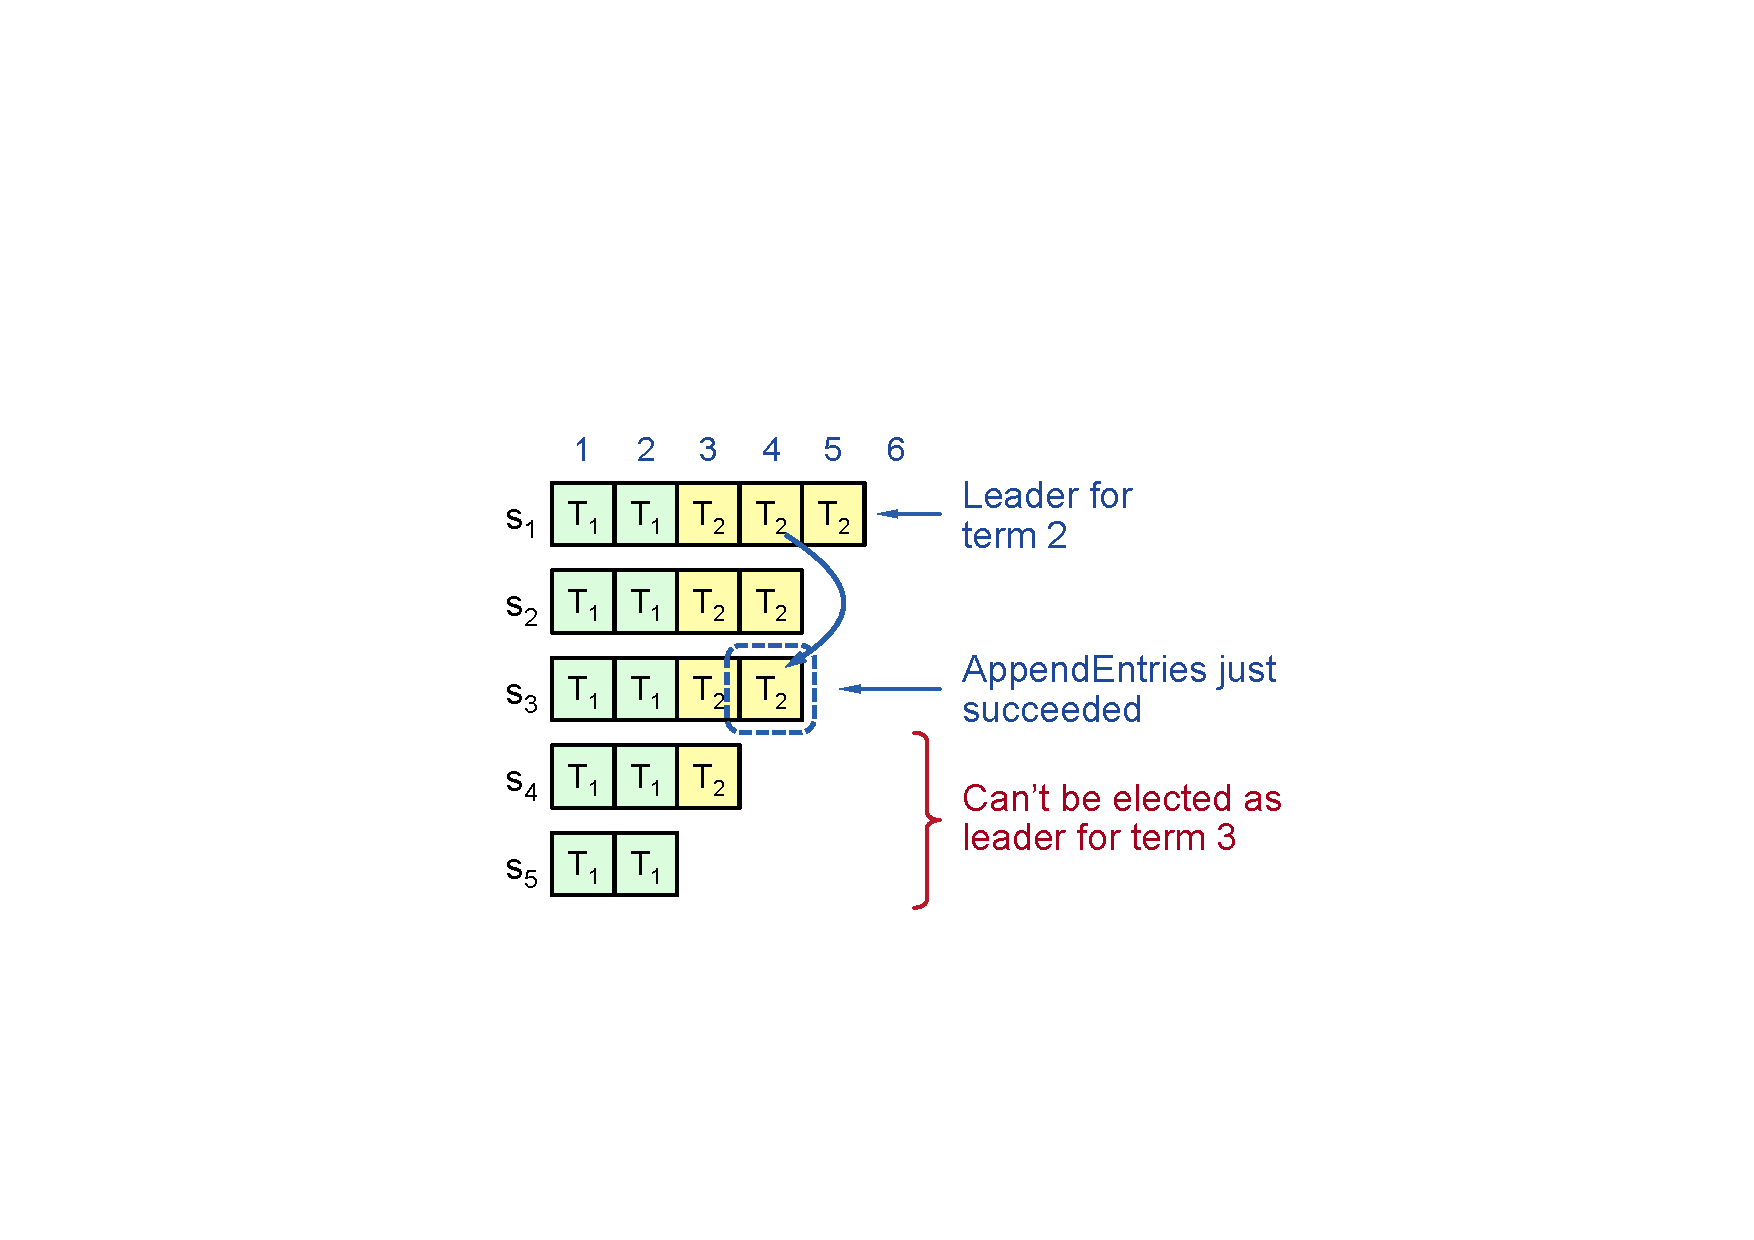
\includegraphics[width=0.5\textwidth]{commit1}
\end{center}

\BB{\alert{Safe}: leader for term $T_3$ must contain entry $T_4$}

\end{frame}

%-------------------------------------------------------------------------
\begin{frame}[t]{Committing Entry from Earlier Terms}


\BB{Case 2/2: Leader is trying to commit entry from an earlier term}

\begin{center}
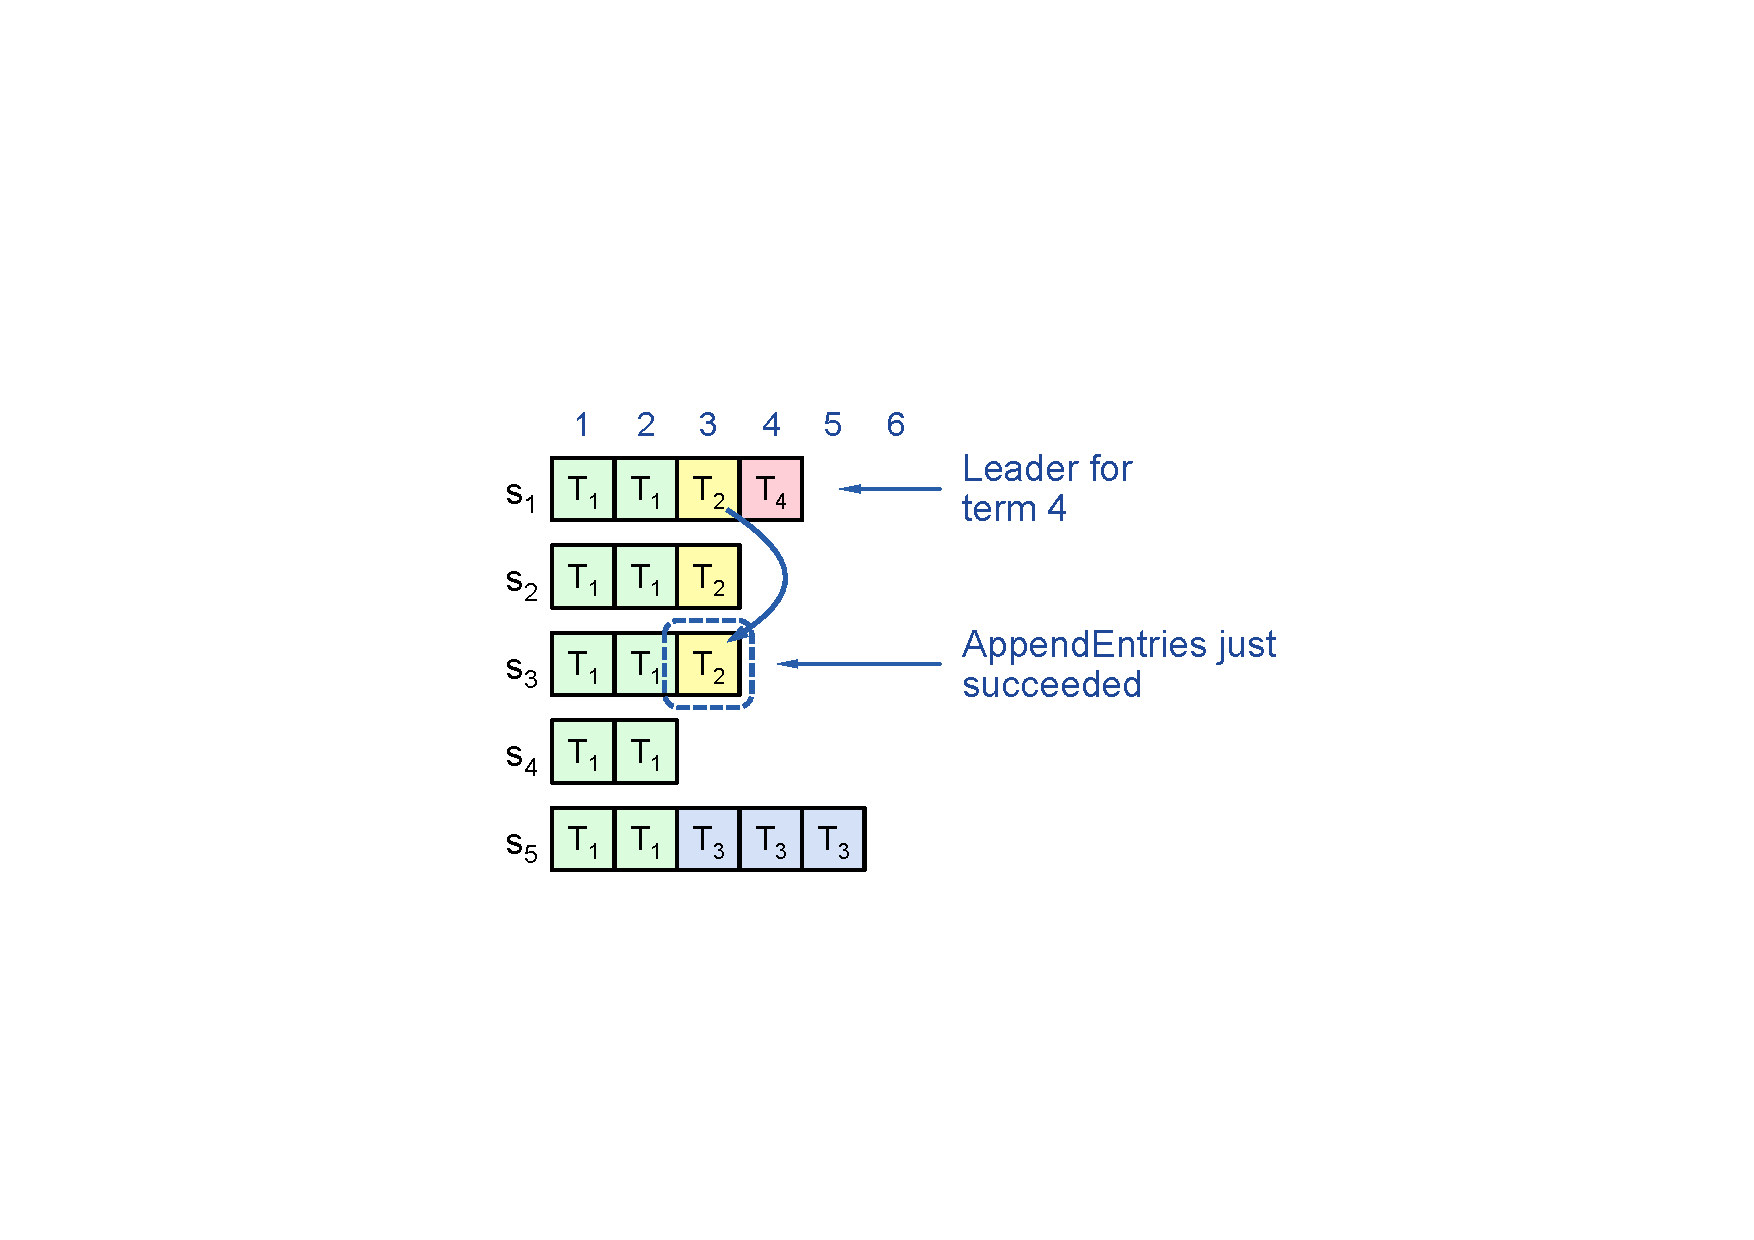
\includegraphics[width=0.5\textwidth]{commit2}
\end{center}

\BB{\alert{Unsafe}: Entry 3 not safely committed}
\BI
\item $s_5$ can be elected as leader for term $T_5$
\item If elected, it will overwrite entry $3$ on $s_1$, $s_2$, and $s_3$!
\EI

\end{frame}


\begin{frame}{New commitment rule}
\begin{columns}[T]
\begin{column}{0.5\textwidth}
\BIL
\item  \alert{For a leader to decide that an entry is committed}:
	\BI
	\item Must be stored on a majority of servers
	\item At least one new entry from leader's term must also be stored on 
			majority of servers
	\EI
\item \alert{Once entry 4 committed}:
	\BI
	\item $s_5$ cannot be elected leader for term $T_5$
	\item Entries 3 and 4 both safe
	\EI
\EIL
\end{column}
\begin{column}{0.5\textwidth}
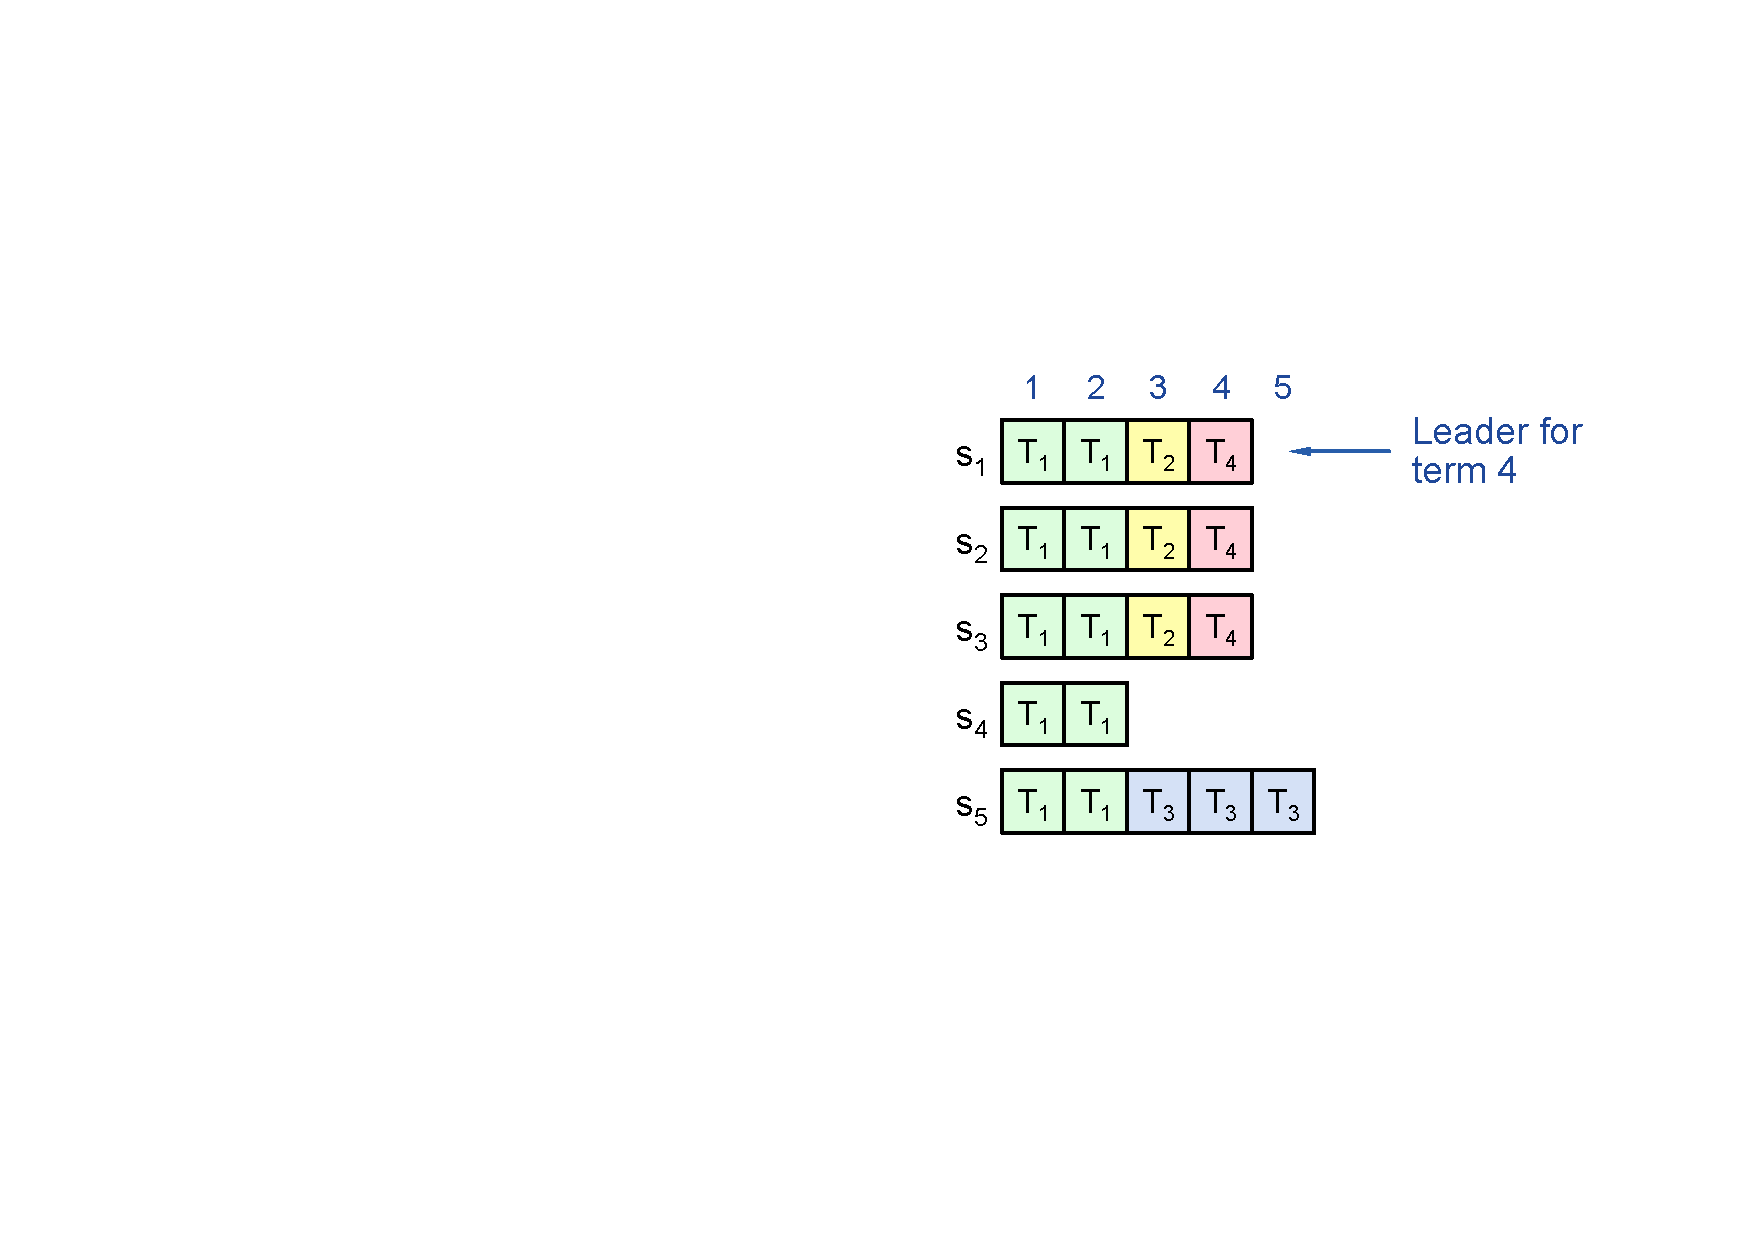
\includegraphics[width=\textwidth]{new-commit}
\end{column}
\end{columns}

\bigskip\bigskip
\BB{Combination of election rules and commitment rules makes Raft safe
}

\end{frame}

%-------------------------------------------------------------------------
\begin{frame}{Log inconsistencies}
	
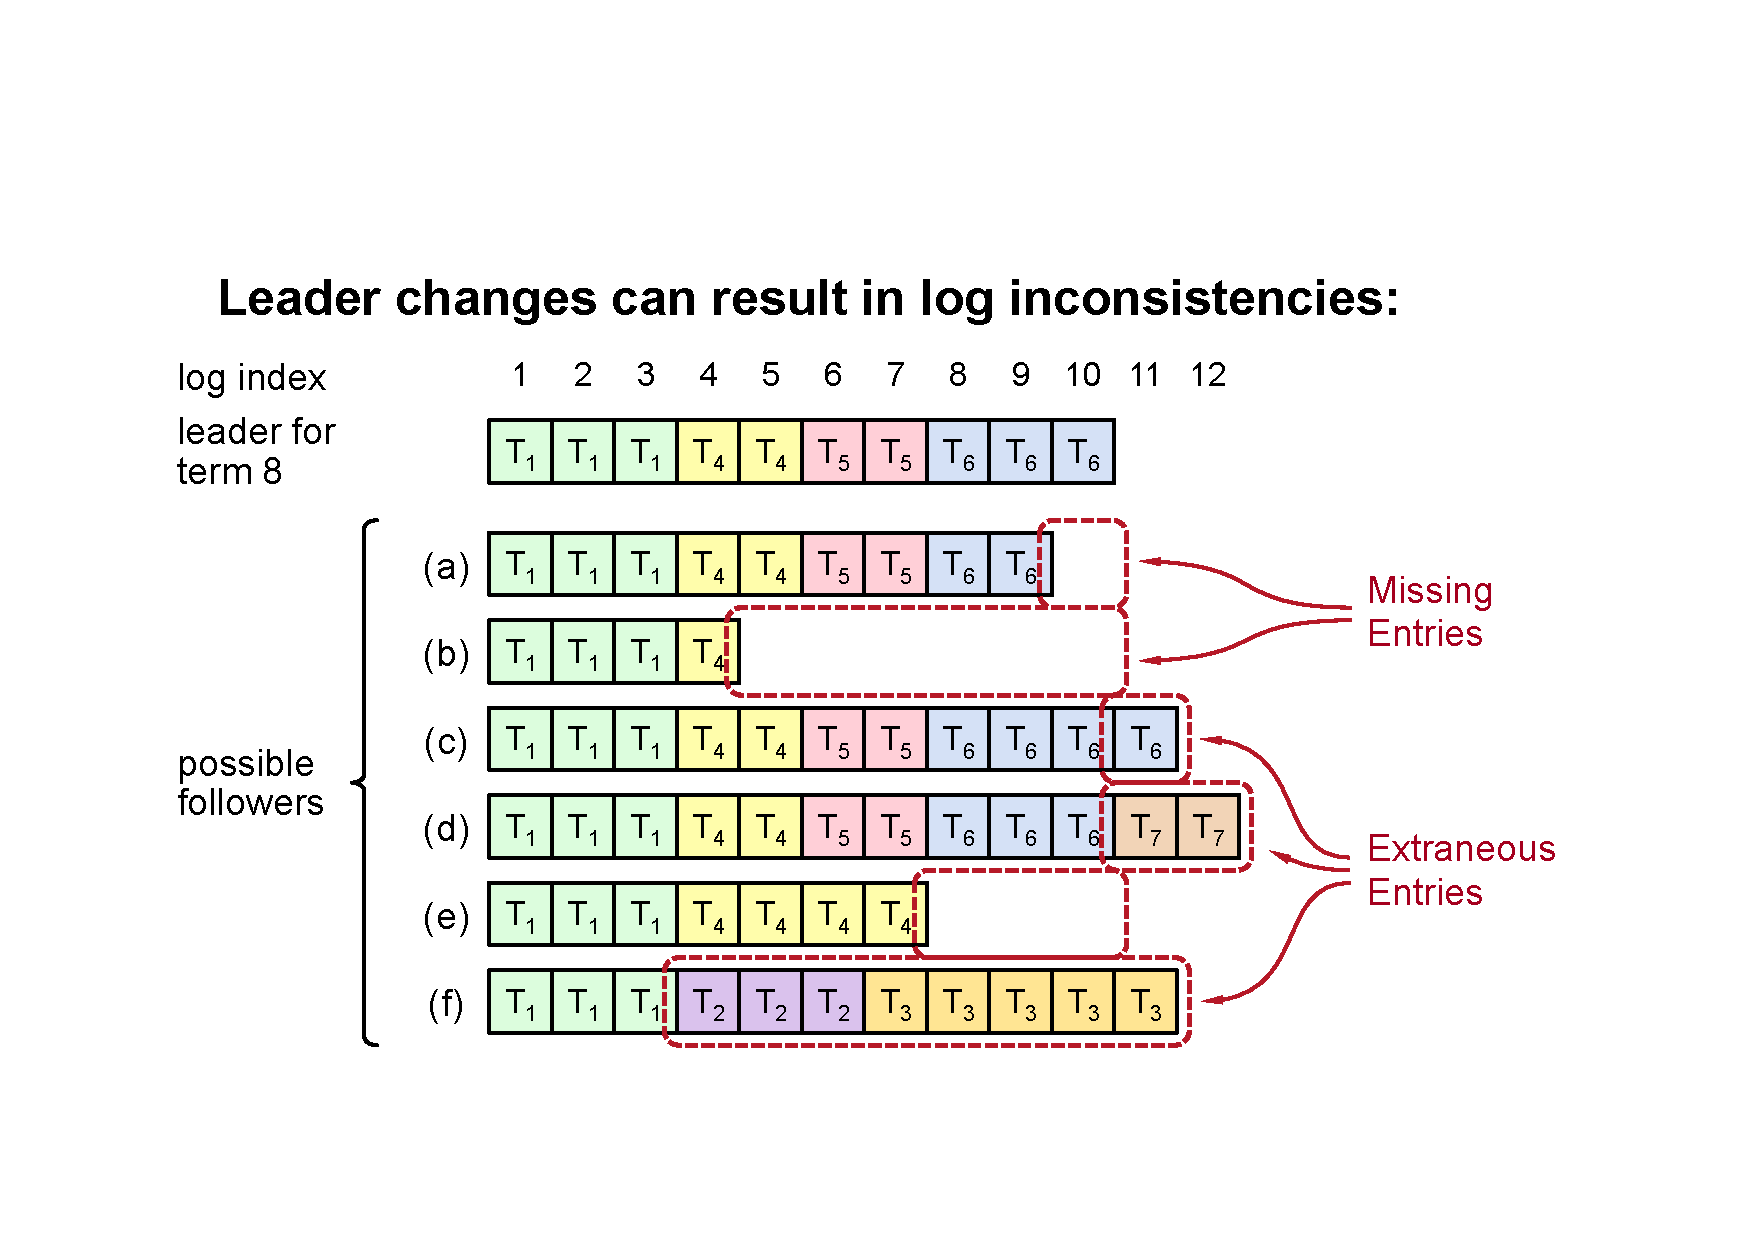
\includegraphics[width=1.0\textwidth]{log-inconsistencies}

\end{frame}

%-------------------------------------------------------------------------
\begin{frame}{Repairing follower log}
\BIL
\item New leader must make follower logs consistent with its own
	\BI
	\item Delete extraneous entries
	\item Fill in missing entries
	\EI
\item  Leader keeps $\nextIndex$ for each follower:
	\BI
	\item Index of next log entry to send to that follower
	\item Initialized to (1 + leader's last index)
	\EI
\item When \AppendRPC consistency check fails, decrement $\nextIndex$ and try again
\EI

\begin{center}
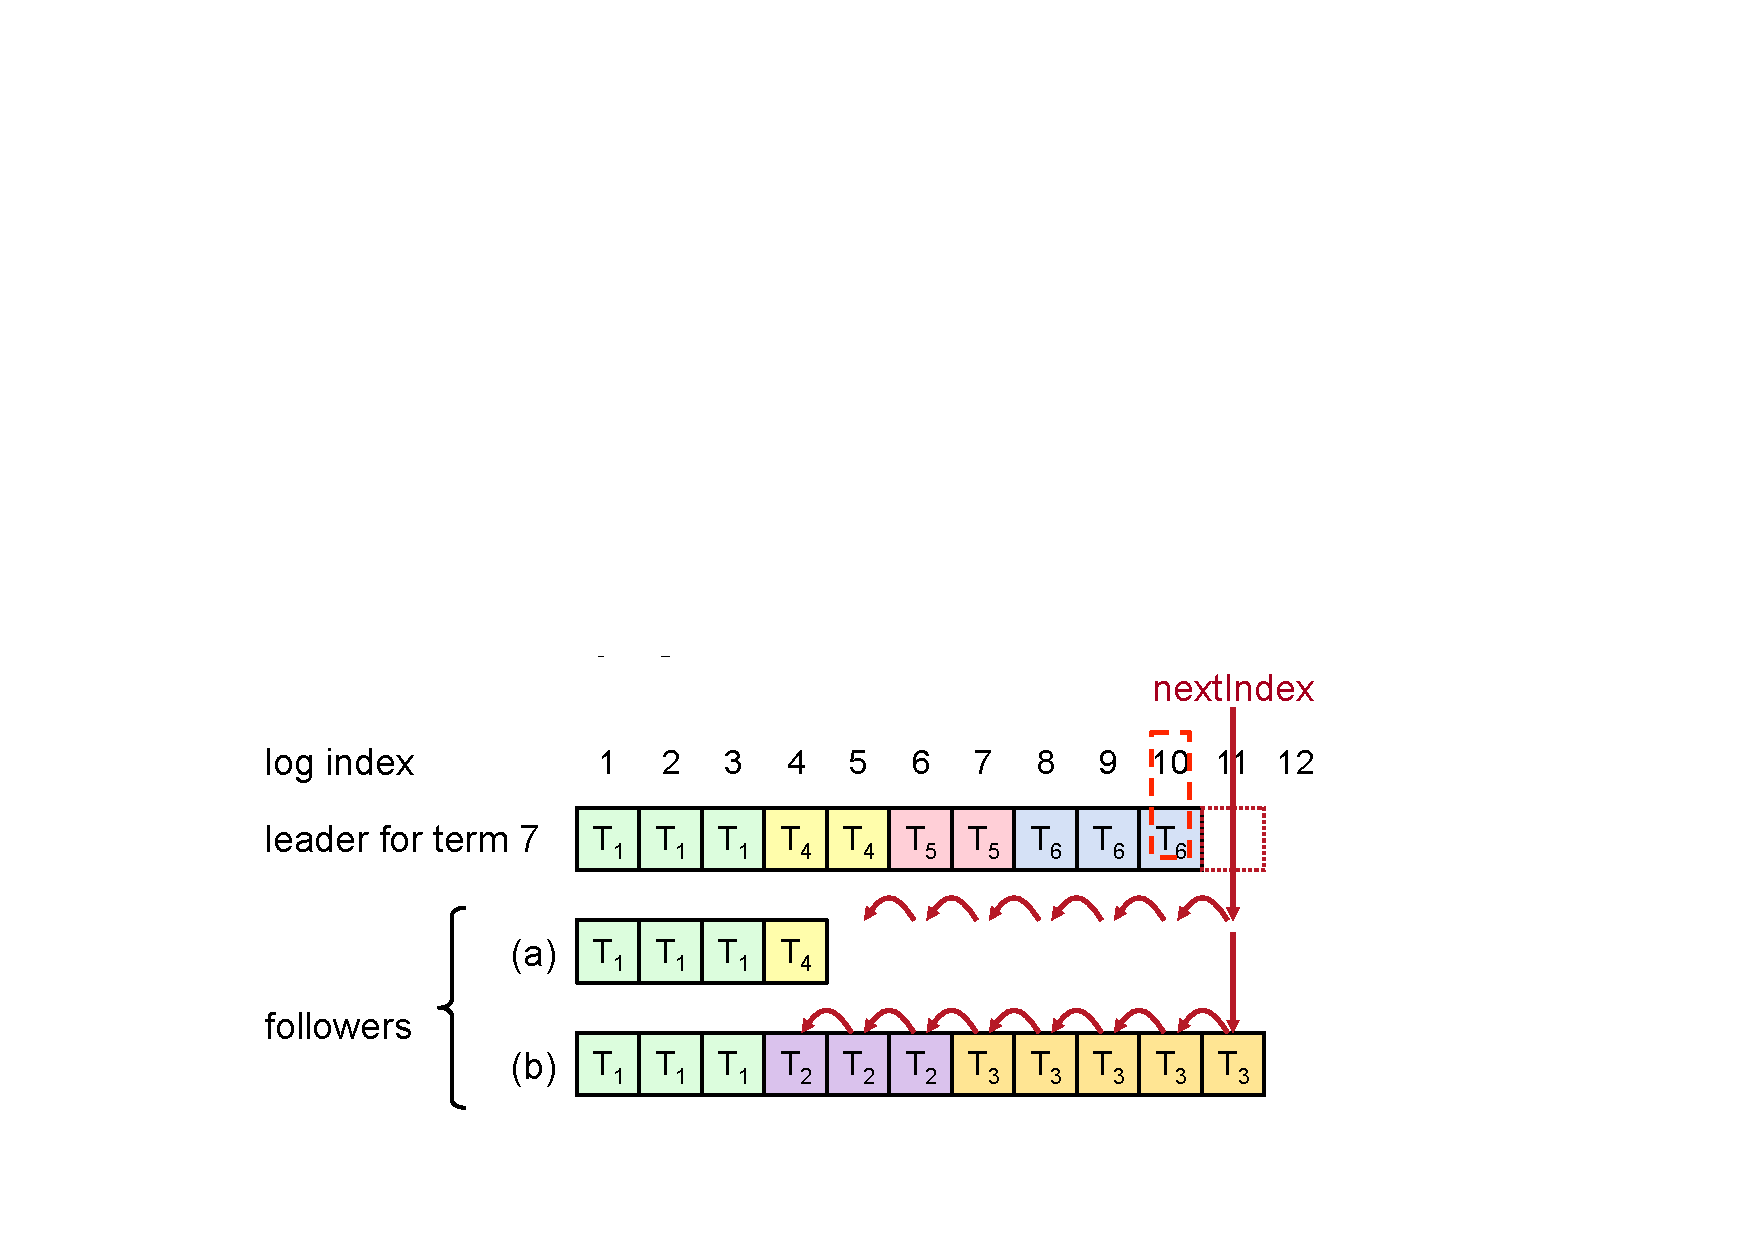
\includegraphics[width=0.6\textwidth]{repair-log1}
\end{center}


\end{frame}

%-------------------------------------------------------------------------
\begin{frame}{Repairing follower log -- Pseudocode}

\begin{Procedure}
\caption{Normal operation code - executed by process $p$}
\UPON{$\RECEIVE \langle \APPENDREPLY, \Term, \Success, \Index \rangle$ \FROM\ $q$}{
  \uIf{$\Term > \CurrentTerm$}{
    $\StepDown(\Term)$\;
  }
  \ElseIf{$\State = \Leader$ \AND\ $\Term = \CurrentTerm$}{
  	\eIf{$\Success$}{
		$\nextIndex[q] \gets \Index+1$\;
	}{
		$\nextIndex[q] \gets \textsf{max}(1,\nextIndex-1$)\;
	}
  	\If{$\nextIndex[q] \leq \log.\Length()$}{
		$\SendAppendEntries(q)$\;
	}
  }
}
\end{Procedure}


\end{frame}

%-------------------------------------------------------------------------
\begin{frame}{Repairing follower log}
	
\BB{When follower overwrites inconsistent entry, it deletes all subsequent entries}

\begin{center}
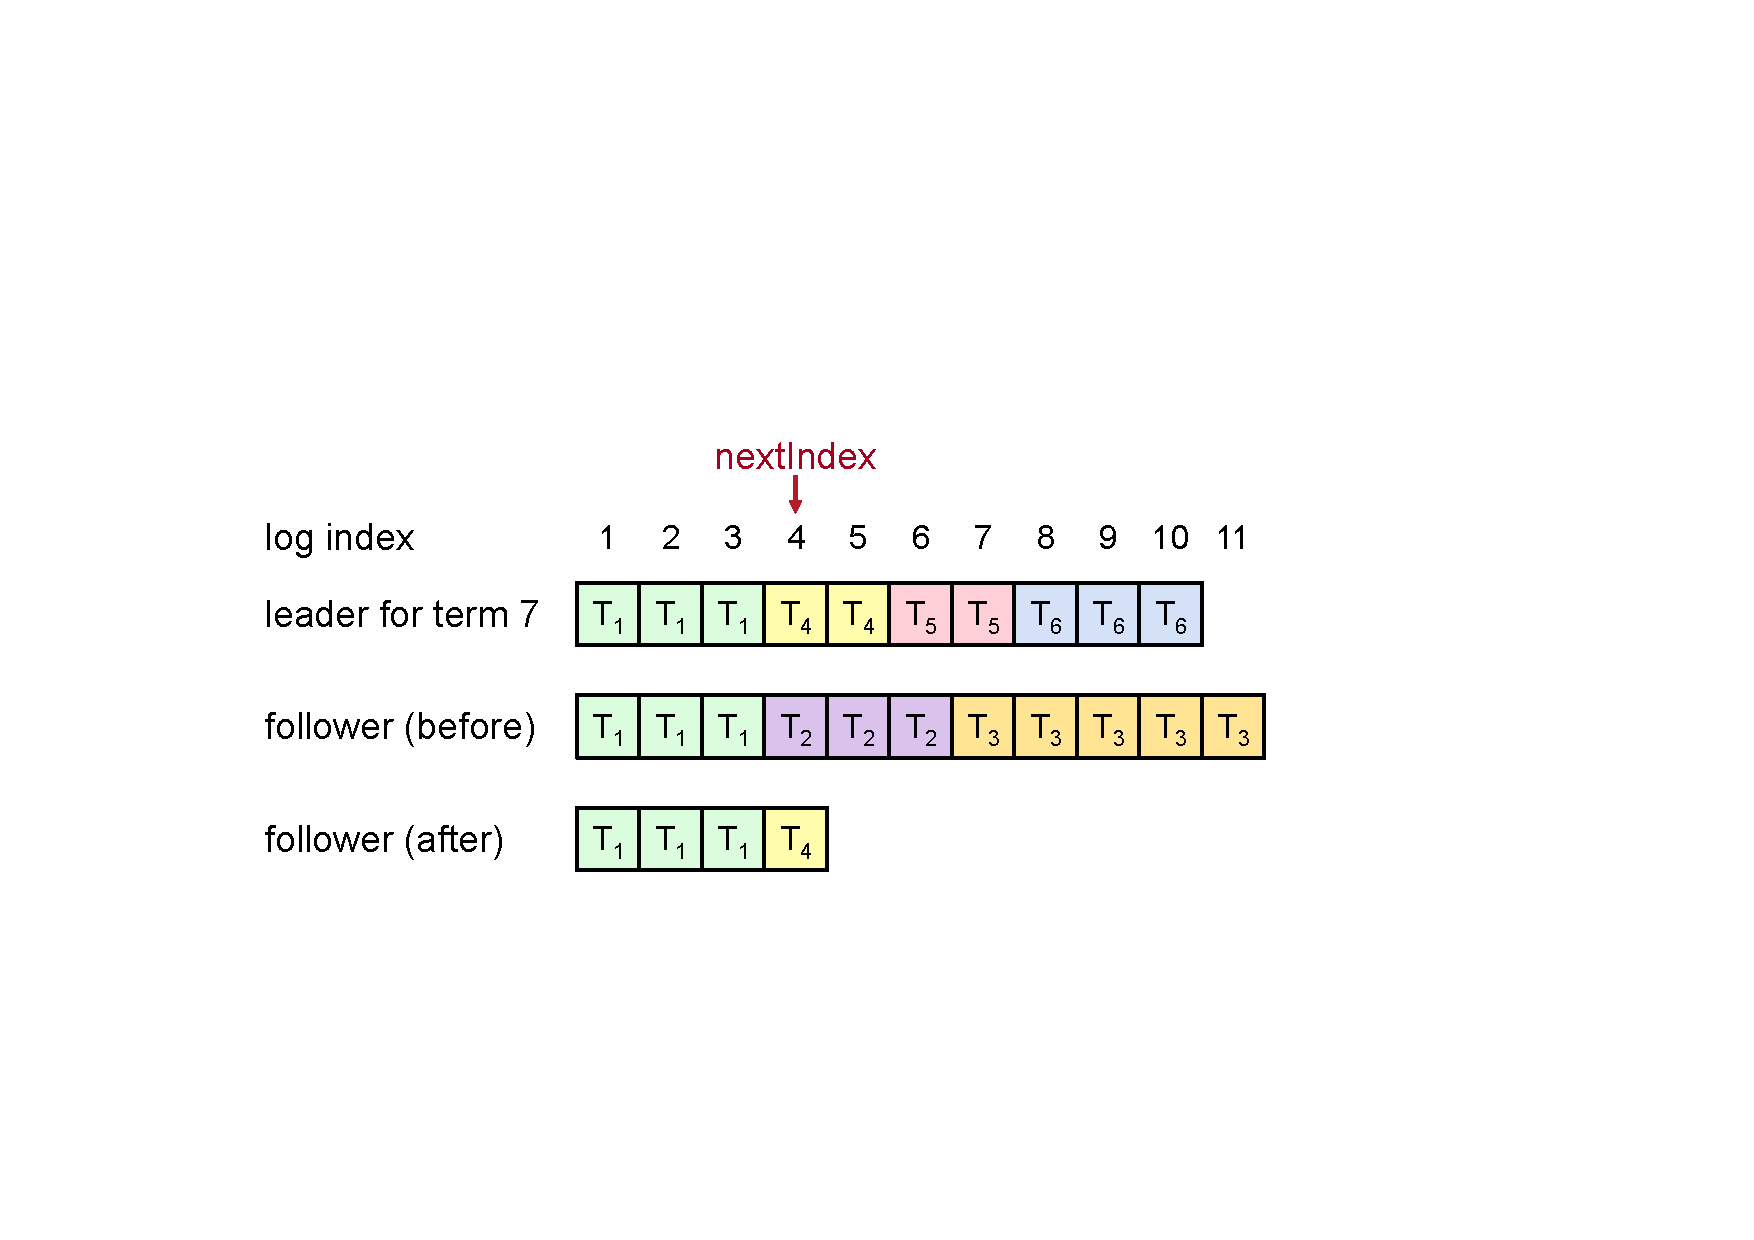
\includegraphics[width=0.8\textwidth]{repair-log2}
\end{center}

	
\end{frame}

\begin{frame}{Repairing follower log}

{
\setlength{\interspacetitleruled}{0pt}%
\setlength{\algotitleheightrule}{0pt}%
\begin{Procedure}
\PROCEDURE{\StoreEntries($\prevIndex, \Entries, c$)}{
$\Index \gets \prevIndex$\;
\For{$j \gets 1$ \TO\ $\Entries.\Length()$}{
	$\Index \gets \Index+1$\;
	\If{$\Log[\Index].\Term \neq \Entries[j].\Term$}{
		$\Log = \Log[1 \ldots \Index-1] + \Entries[j]$\;
	}
}
$\commitIndex \gets \textsf{min}(c, \Index)$\;
\Return $\Index$\;
}
\end{Procedure}	
}
	
\end{frame}

%%%%%%%%%%%%%%%%%%%%%%%%%%%%%%%%%%%%%%%%%%%%%%%%%%%%%%%%%%%%%%%%%%%%%%%%%%

\subsection{Neutralizing old leaders}

%-------------------------------------------------------------------------
\begin{frame}{Neutralizing Old Leaders}
	
\BB{Deposed leader may not be dead}
	\BI
	\item Temporarily disconnected from network
	\item Other servers elect a new leader
	\item Old leader becomes reconnected, attempts to commit log entries
	\EI

\medskip
\BB{Terms used to detect stale leaders (and candidates)}
	\BI
	\item Every RPC contains term of sender
	\item If sender's term is older, RPC is rejected, sender reverts to follower and updates its term
	\item If receiver's term is older, it reverts to follower, updates its term, then processes RPC normally
	\EI

\medskip
\BB{Election updates terms of majority of servers}
	\BI
	\item Deposed server cannot commit new log entries
	\EI

	
\end{frame}


%-------------------------------------------------------------------------
\begin{frame}{Neutralizing Old Leaders}
	
\begin{Procedure}
\caption{Normal operation code - executed by process $p$}
\ONRECEIVE{$\langle \APPENDREQUEST, \Term, \prevIndex, \prevTerm, \ldots \rangle$ \FROM $q$}{
  \If{$\Term > \CurrentTerm$}{
    $\StepDown(\Term)$\;
  }
  \eIf{$\Term < \CurrentTerm$}{
    \SEND $\langle \APPENDREPLY, \CurrentTerm, \FALSE \rangle$ \TO\ $q$
  }{
  	[\ldots]\;
  }
}
\end{Procedure}
\end{frame}

\subsection{Client protocol}

%-------------------------------------------------------------------------
\begin{frame}{Client protocol}

\BB{Clients sends commands to leader:}
	\BI
	\item If leader unknown, contact any server
	\item If contacted server not leader, it will redirect to leader
	\EI
	
\BB{Leader responds when:}
	\BI
	\item command has been logged
	\item command has been committed
	\item command has been executed by leader's state machine
	\EI
	
\BB{If request times out (e.g., leader crash):}
	\BI
	\item Client re-issues command to some other server
	\item Eventually redirected to new leader
	\item Retry request with new leader
	\EI

\end{frame}

%-------------------------------------------------------------------------
\begin{frame}{Client protocol}

\BB{What if leader crashes after executing command, but before responding?}
\BI
\item Must not execute command twice
\EI

\BB{Solution: client embeds a unique id in each command}
\BI
\item Server includes id and response in log entry
\item Before accepting command, leader checks its log for entry with that id
\item If id found in log, ignore new command, return response from old command
\EI

\BB{Result: exactly-once semantics as long as client doesn't crash}

\end{frame}

\subsection{Configuration changes}

%-------------------------------------------------------------------------
\begin{frame}{Configuration}

\begin{block}{System configuration}	
\BI
\item ID, address for each server
\item Determines what constitutes a majority
\EI
\end{block}

\bigskip
\BB{Consensus mechanism must support changes in the configuration}
\BI
\item Replace failed machine
\item Change degree of replication
\EI

\end{frame}
%-------------------------------------------------------------------------
\begin{frame}{Configuration changes}

\BB{Cannot switch directly from one configuration to another: \\
conflicting majorities could arise}

\begin{center}
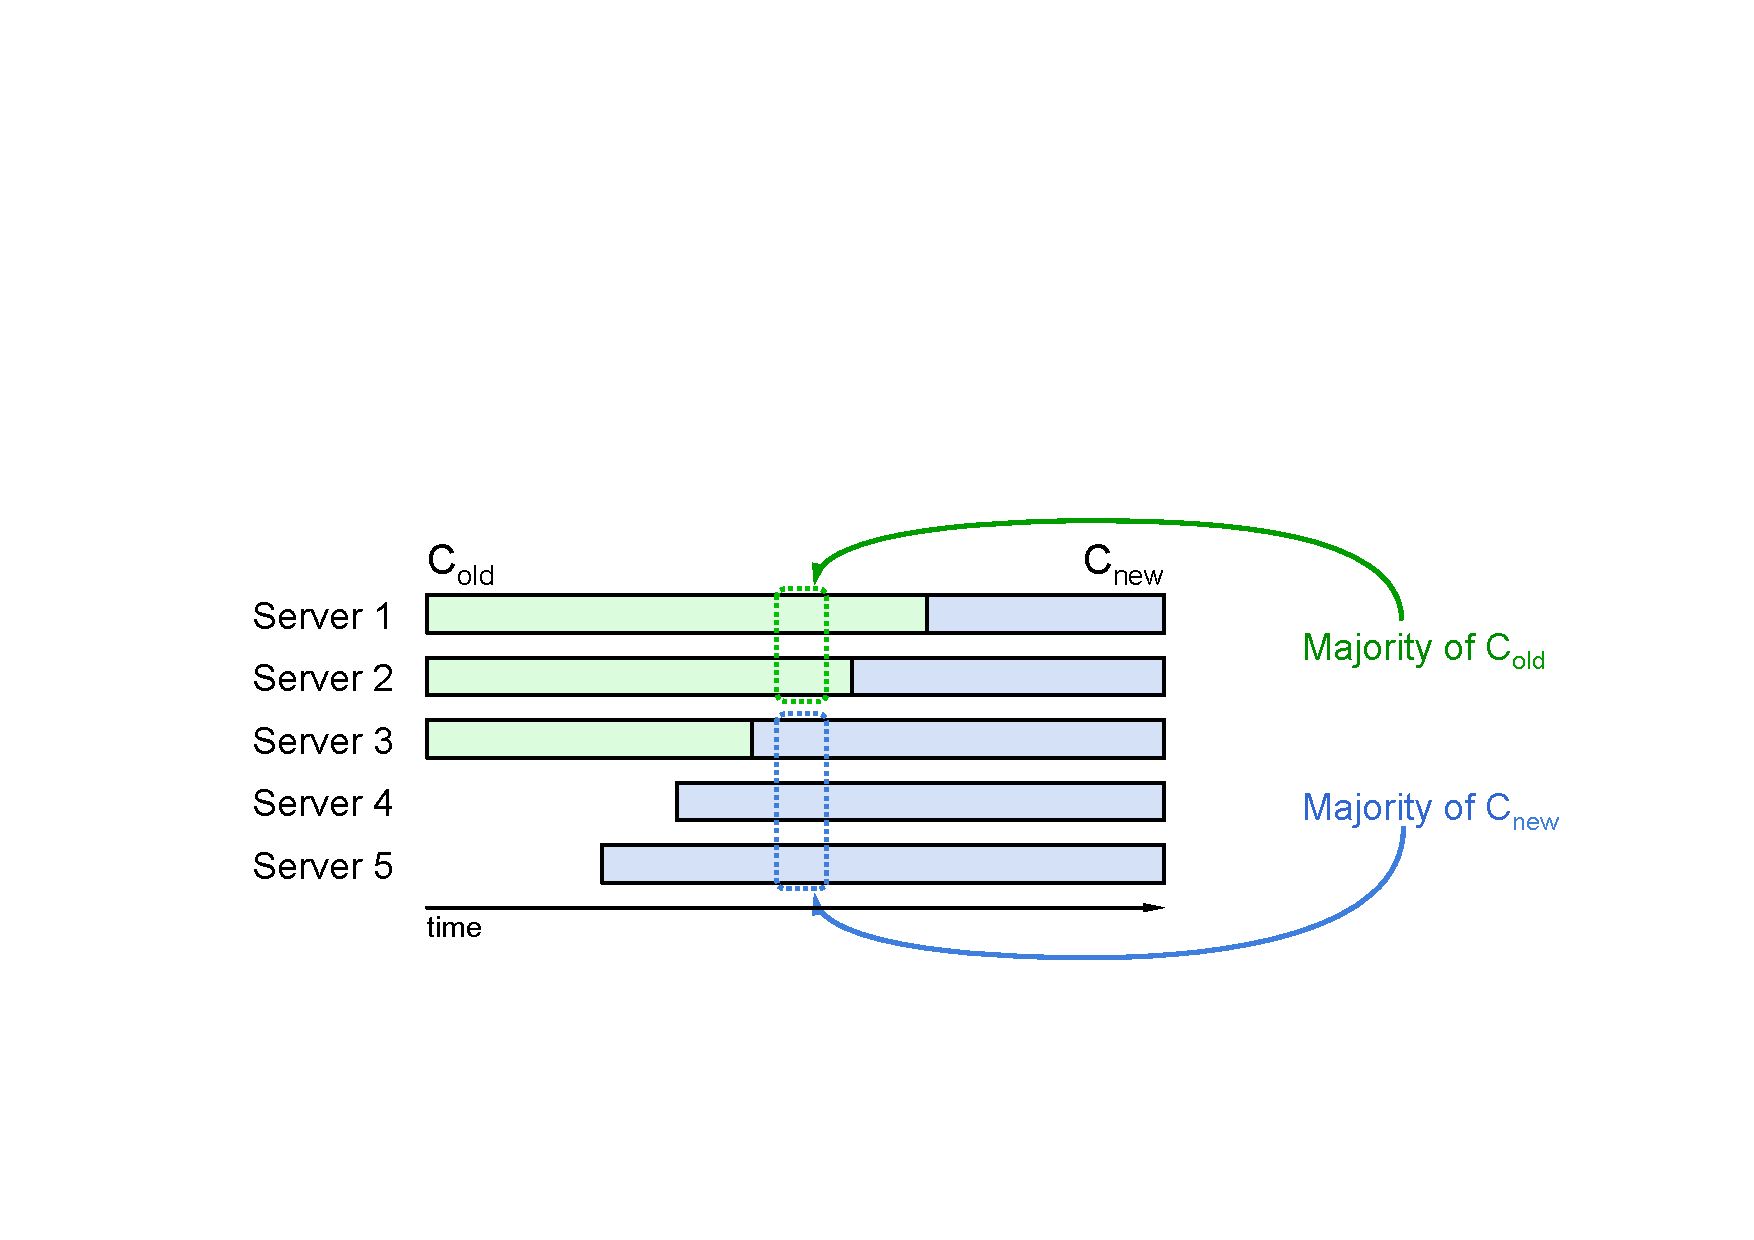
\includegraphics[width=\textwidth]{configuration-changes}
\end{center}

\end{frame}
%-------------------------------------------------------------------------
\begin{frame}{Joint consensus}
\BB{Raft uses a 2-phase approach}
\BIL
\item Intermediate phase uses joint consensus (need majority of both old and new configurations for elections, commitment)
\item Once joint consensus is committed, begin replicating log entry for final configuration
\EIL

\begin{center}
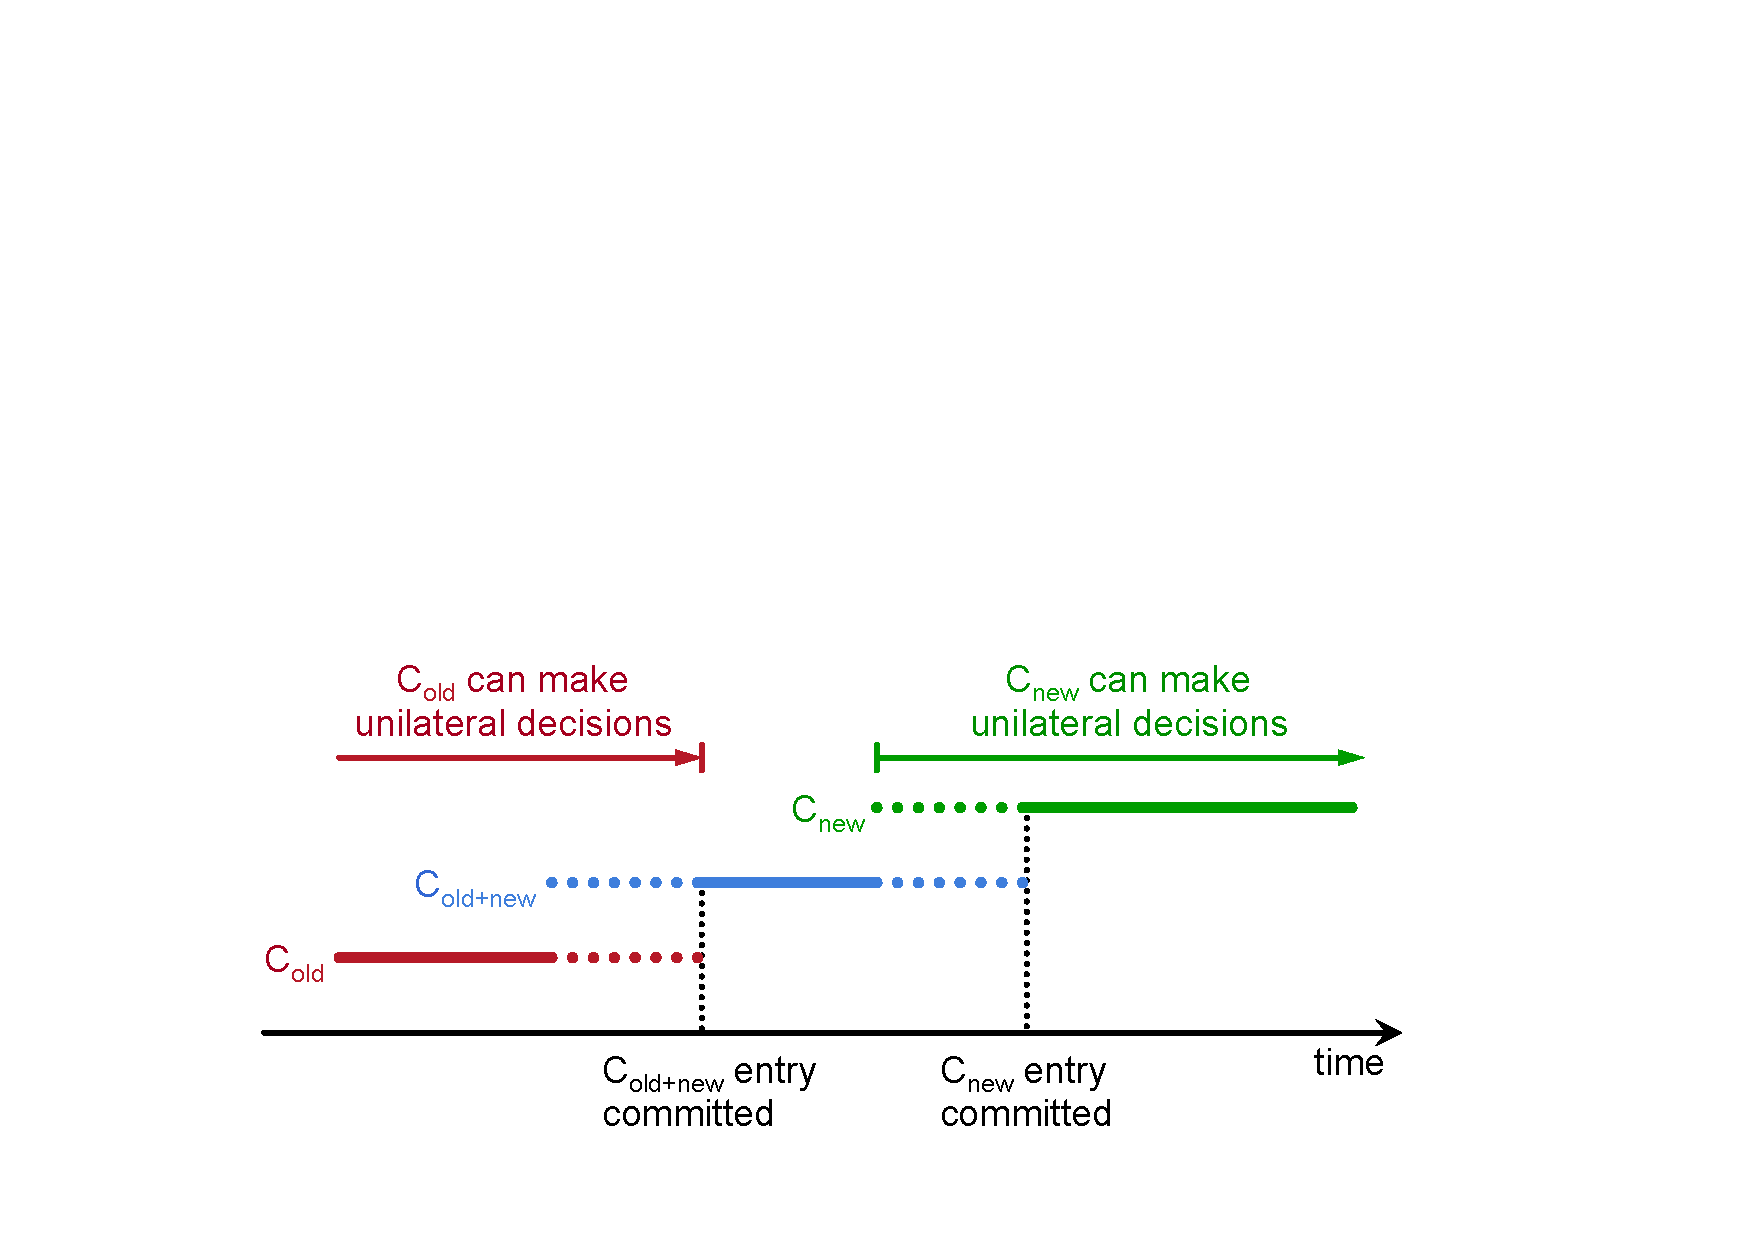
\includegraphics[width=0.8\textwidth]{joint-consensus}
\end{center}

\end{frame}



%-------------------------------------------------------------------------
\begin{RMFrame}

\BI
\item \bibentry{raft}
\EI

\end{RMFrame}


\end{document}

%-------------------------------------------------------------------------
\begin{frame}{}
\end{frame}
